%% This is a monograph which uses `coppe' document
%% class and `coppe-unsrt' BibTeX style.
%% 
%% \CheckSum{1648}
%% \CharacterTable
%%  {Upper-case    \A\B\C\D\E\F\G\H\I\J\K\L\M\N\O\P\Q\R\S\T\U\V\W\X\Y\Z
%%   Lower-case    \a\b\c\d\e\f\g\h\i\j\k\l\m\n\o\p\q\r\s\t\u\v\w\x\y\z
%%   Digits        \0\1\2\3\4\5\6\7\8\9
%%   Exclamation   \!     Double quote  \"     Hash (number) \#
%%   Dollar        \$     Percent       \%     Ampersand     \&
%%   Acute accent  \'     Left paren    \(     Right paren   \)
%%   Asterisk      \*     Plus          \+     Comma         \,
%%   Minus         \-     Point         \.     Solidus       \/
%%   Colon         \:     Semicolon     \;     Less than     \<
%%   Equals        \=     Greater than  \>     Question mark \?
%%   Commercial at \@     Left bracket  \[     Backslash     \\
%%   Right bracket \]     Circumflex    \^     Underscore    \_
%%   Grave accent  \`     Left brace    \{     Vertical bar  \|
%%   Right brace   \}     Tilde         \~}
%%
\documentclass[msc]{coppe}

\usepackage{booktabs}% tabelas mais bonitas
\usepackage{rotating}% rodando coisas, como tabelas
\usepackage{longtable} % tabelas longas
\usepackage[most]{tcolorbox} % caixas de texto
\usepackage{amsmath,amssymb}
\usepackage{hyperref}

\usepackage{multirow}
\usepackage{changepage} 

\usepackage{adjustbox} 

\usepackage{xcolor, colortbl} % For more complex coloring of cells
\usepackage{hhline} % For double lines

\usepackage{algorithm}
% \usepackage{algorithmic}
\usepackage{algpseudocode}

\usepackage{lmodern}
\usepackage[T1]{fontenc}

\usepackage{silence}
% \WarningFilter{latex}{Overfull}
\WarningFilter{latex}{Underfull}

% \usepackage{float}
\usepackage{pdflscape} % in preamble

% \usepackage[a4paper,margin=1.5cm]{geometry}


\makelosymbols
\makeloabbreviations

\begin{document}


\title{Comparative Analysis of Single and Multi-Agent Large Language Model Architectures for Domain-Specific Tasks in Well Construction}
\foreigntitle{Comparative Analysis of Single and Multi-Agent Large Language Model Architectures for Domain-Specific Tasks in Well Construction}
\author{Vitor}{Brandão Sabbagh}
\advisor{Prof.}{Geraldo}{Bonorino Xexéo}{D.Sc.}

\examiner{Prof.}{Nome do Primeiro Examinador Sobrenome}{D.Sc.}
\examiner{Prof.}{Nome do Segundo Examinador Sobrenome}{Ph.D.}
\examiner{Prof.}{Nome do Terceiro Examinador Sobrenome}{D.Sc.}
\examiner{Prof.}{Nome do Quarto Examinador Sobrenome}{Ph.D.}
\examiner{Prof.}{Nome do Quinto Examinador Sobrenome}{Ph.D.}
\department{PESC}
\date{07}{2025}

\keyword{Large Language Models}
\keyword{Agentes}
\keyword{Construção de Poços de Petroleo}

\maketitle

\frontmatter
\dedication{Para Carolina, minha companheira de vida.}

\chapter*{Agradecimentos}

Gostaria de agradecer a todos. [família, amigos, etc]

Estendo minha gratidão aos especialistas em engenharia de poços, Marcelo Grimberg, Rafael Peralta e Lorenzo Simonassi, cuja expertise e dedicação contribuíram significativamente para esta pesquisa.


\begin{abstract}

Apresenta-se, nesta tese, a aplicação de grandes modelos de linguagem (LLM) no setor de petróleo e gás, especificamente em tarefas de construção e manutenção de poços. O estudo avalia o desempenho de uma arquitetura baseada em LLM de agente único e de múltiplos agentes no processamento de diferentes tarefas, oferecendo uma perspectiva comparativa sobre sua precisão e as implicações de custo de sua implementação. Os resultados indicam que sistemas multiagentes oferecem desempenho melhorado em tarefas de perguntas e respostas, com uma medida de veracidade 28\% maior do que os sistemas de agente único, mas a um custo financeiro mais alto. Especificamente, a arquitetura multiagente incorre em custos que são, em média, 3,7 vezes maiores do que os da configuração de agente único, devido ao aumento do número de tokens processados. Por outro lado, os sistemas de agente único se destacam em tarefas de texto para SQL (Linguagem de Consulta Estruturada), especialmente ao usar o Transformador Pré-Treinado Generativo 4 (GPT-4), alcançando uma pontuação 15\% maior em comparação com as configurações multiagentes, sugerindo que arquiteturas mais simples podem, às vezes, superar a complexidade. A novidade deste trabalho reside em seu exame original dos desafios específicos apresentados pelos dados complexos, técnicos e não estruturados inerentes às operações de construção de poços, contribuindo para o planejamento estratégico da adoção de aplicações de IA generativa, fornecendo uma base para otimizar soluções contra parâmetros econômicos e tecnológicos.

\end{abstract}

\begin{foreignabstract}


This article explores the application of large language models (LLM) in the oil and gas  sector, specifically within well construction and maintenance tasks. The study evaluates the performances of a single-agent and a multi-agent LLM-based architecture in processing different tasks, offering a comparative perspective on their accuracy and the cost implications of their implementation. The results indicate that multi-agent systems offer improved performance in question and answer tasks, with a truthfulness measure 28\% higher than single-agent systems, but at a higher financial cost. Specifically, the multi-agent architecture incurs costs that are, on average, 3.7 times higher than those of the single-agent setup due to the increased number of tokens processed. Conversely, single-agent systems excel in text-to-SQL (Structured Query Language) tasks, particularly when using Generative Pre-Trained Transformer 4 (GPT-4), achieving a 15\% higher score compared to multi-agent configurations, suggesting that simpler architectures can sometimes outpace complexity. The novelty of this work lies in its original examination of the specific challenges presented by the complex, technical, unstructured data inherent in well construction operations, contributing to strategic planning for adopting generative AI applications, providing a basis for optimizing solutions against economic and technological parameters. 

\end{foreignabstract}

\tableofcontents
\listoffigures
\listoftables
\printlosymbols
\printloabbreviations

\mainmatter




\chapter{Introdução}

% Segundo a norma de formatação de teses e dissertações do
% Instituto Alberto Luiz Coimbra de Pós-graduação e Pesquisa de
% Engenharia (COPPE), toda abreviatura deve ser definida antes de
% utilizada.\abbrev{COPPE}{Instituto Alberto Luiz Coimbra de Pós-gradua{\c
% c}\~ao e Pesquisa de Engenharia}.

% Do mesmo modo, é imprescindível definir os símbolos, tal como o
% conjunto dos números reais $\mathbb{R}$ e o conjunto vazio $\emptyset$.
% \symbl{$\mathbb{R}$}{Conjunto dos números reais}
% \symbl{$\emptyset$}{Conjunto vazio}

% Para as listas de abreviaturas e símbolos funcionarem, é necessário rodar o \verb|latexmkrc|. O Overleaf faz isso automaticamente. Caso haja um problema, verifique se o arquivo \verb|coppe.ist| está no diretório. Também é útil compilar do início e apagar todos os arquivos desnecessários.


\section{Contextualização}

% [IA-GEN NA INDÚSTRIA]
Na dinâmica em constante mudança da indústria de petróleo e gás (O\&G), a transformação digital emergiu como um elemento chave para alcançar eficiência operacional, sustentabilidade e competitividade.
Na vanguarda dessa transformação estão os Modelos de Linguagem de Grande Escala (LLMs), que têm o potencial de processar consultas não estruturadas, mapear alternativas e aconselhar os usuários sobre possíveis ações \cite{Kar2023}.
Também observamos a vantagem do aumento do engajamento, cooperação, acessibilidade e, em última análise, lucratividade.
Esses modelos redefinem paradigmas em gestão do conhecimento e recuperação de informações e impactam uma variedade de outras áreas \cite{Eckroth2023}, tornando crucial a adoção dessas tecnologias para permanecer competitivo.

% [ESTUDO AUMENTO PRODUTIVIDADE]
Um estudo conduzido por \cite{Dellacqua2023}, em colaboração com o Boston Consulting Group, demonstra que em tarefas intensivas em conhecimento, consultores equipados com acesso a LLMs como o GPT-4 não apenas completaram as tarefas mais eficientemente (25,1\% mais rapidamente em média), mas também com qualidade substancialmente maior, alcançando resultados mais de 40\% melhores em comparação com aqueles sem assistência de IA \cite{Dellacqua2023}. O aumento da produtividade dos trabalhadores do conhecimento foi de 12\% em média.
Para ilustrar, se considerarmos os \$2,8 bilhões gastos em remuneração por uma grande empresa de petróleo, dos quais 60\% vão para trabalhadores do conhecimento (\$1,6 bilhões), um aumento de 12\% na produtividade poderia ser visto como gerando um valor adicional de \$204 milhões em produção da mesma força de trabalho.
% [AUMENTO DO PIB DEVIDO A GEN AI]
Indicadores econômicos mais amplos preveem transformações significativas devido à IA generativa (Gen-AI) em vários setores.
Um relatório do Goldman Sachs \cite{Hatzius2023} destaca que a Gen-AI está prestes a aumentar o PIB global em quase 7\%, aumentando o crescimento da produtividade em 1,5 pontos percentuais na próxima década.

\section{Motivação}
% [PROBLEMA DE DADOS NA INDÚSTRIA EM GERAL]
Expandindo a discussão mais ampla sobre a utilização de dados nas organizações, um problema importante é o desafio de extrair informações relevantes de extensas bases de dados \cite{Singh2023}.
Inicialmente, o desafio de conhecer, encontrar e acessar dados representa um obstáculo significativo para os processos de tomada de decisão. Colaboradores em empresas de O\&G frequentemente enfrentam a tarefa intensiva de buscar manualmente em grandes repositórios de dados para encontrar informações úteis.

% [PROBLEMA DE DADOS NO O&G]
Focando especificamente nas atividades de perfuração e completação de poços offshore e onshore, um grande desafio reside na natureza inerentemente complexa e técnica dos dados envolvidos, que podem ser de vários tipos: operações, projetos, tecnologias, cadeias de suprimentos e outros.
A ineficiência em aproveitar grandes volumes de dados não estruturados agrava esses desafios, como observado por \cite{Singh2023}. Uma quantidade significativa dos dados gerados e coletados neste setor é não estruturada, variando de relatórios de texto e e-mails a imagens e vídeos de atividades de exploração e produção.
As empresas de O\&G enfrentam desafios na extração de informações relevantes de vastos dados não estruturados, impactando a tomada de decisões e a inovação \cite{Singh2023}.
Exemplos incluem centenas de relatórios operacionais diários de sondas de perfuração, projetos de execução de poços, relatórios de tempo não produtivo (NPT) e documentos de lições operacionais aprendidas, conforme ilustrado na Figura \ref{fig:report_example}.
Como resultado, informações valiosas podem permanecer inexploradas e o potencial para encontrar insights, tomar decisões informadas e inovar é significativamente comprometido.
\cite{Singh2023} destaca as capacidades e o potencial de chatbots habilitados por IA Generativa para o setor de O\&G, particularmente em melhorar a análise de perfuração e produção para alcançar melhores resultados de negócios. O autor conclui que as empresas que adotarem essas tecnologias nos próximos anos verão vantagens claras.

\begin{figure}[t]
  \centering
  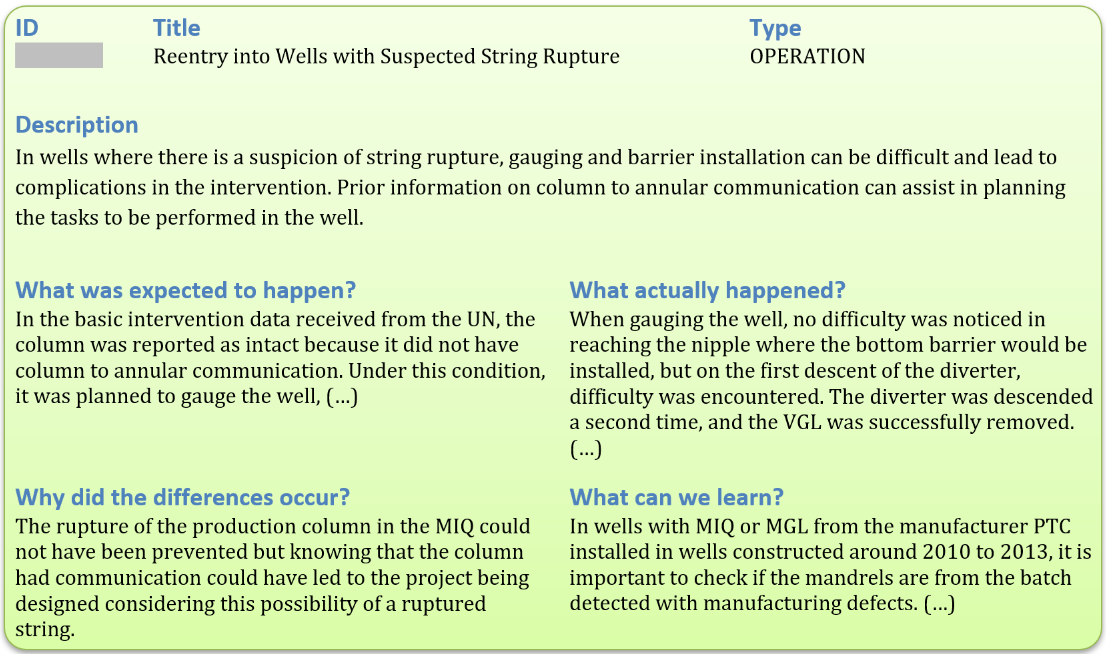
\includegraphics[width=1\textwidth]{images/report_example.png}
  \caption{Amostra de lição aprendida de perfuração e completação. Documento parcial de uma grande empresa de petróleo. (traduzido do português)}
  \label{fig:report_example}
\end{figure}

A implantação de tecnologias de IA enfrenta desafios como dados tendenciosos, alucinações e falta de explicabilidade \cite{Hadi2023}, necessitando de uma abordagem equilibrada. Embora pesquisas anteriores tenham abordado amplamente a IA na indústria, este estudo examina de forma única os desafios e soluções para dados não estruturados complexos em operações de O\&G. Este trabalho aborda a lacuna na compreensão do desempenho de arquiteturas LLM de agente único versus multi-agente em tarefas específicas de domínio, como engenharia de poços, oferecendo insights sobre sua eficácia e relação custo-benefício. A adoção de LLM por uma grande empresa de petróleo destaca o potencial dessas tecnologias para transformar a análise e gestão de dados.

\section{Objetivos}

Esta pesquisa aborda diretamente os desafios enfrentados por grandes empresas de petróleo. Ao investigar as vantagens comparativas e limitações de várias arquiteturas de IA generativa (Gen-AI), incluindo sistemas de agente único e multiagente, este estudo visa identificar as soluções mais eficientes e econômicas.
Os objetivos específicos desta pesquisa são avaliar a adequação e eficácia dos sistemas multiagentes baseados em LLMs para tarefas complexas e específicas de domínios na engenharia de poço, com o objetivo de otimizar o acesso à informação e a tomada de decisões.
O estudo compara sistemas de IA de agente único e multiagente em termos de sua capacidade de responder a consultas relacionadas à engenharia de poços. Ele também mapeia os possíveis obstáculos e limitações associados à implantação de aplicações de Gen-AI.

Os insights obtidos com esta pesquisa visam contribuir diretamente para os objetivos estratégicos das empresas de O\&G, melhorando o acesso a informações sobre engenharia de poços e tarefas de análise de dados automatizadas.
Uma compreensão abrangente dos desafios e limitações associados à Gen-AI permitirá decisões informadas sobre sua adoção, maximizando o retorno sobre o investimento.

\section{Delimitação do Escopo de Negócio}

Para contextualizar o escopo deste estudo, é necessário entender o ciclo de vida de um campo de petróleo, que começa com a Exploração, progride para o Desenvolvimento da Produção, segue com a produção efetiva e culmina no descomissionamento \cite{Badiru2016}. A construção de poços, que envolve a perfuração e completação de poços para extração de hidrocarbonetos, é uma atividade dentro da fase de Desenvolvimento da Produção \cite{Thomas2004}. A Gen-AI tem o potencial de impactar cada uma dessas fases, mas o foco deste trabalho está nas operações das fases de desenvolvimento e manutenção.

A construção de poços é uma atividade altamente especializada que envolve a perfuração e completação de poços para extração de hidrocarbonetos \cite{Thomas2004}. Neste contexto, a Gen-AI pode ser aplicada de várias maneiras. Por exemplo, um chatbot pode gerenciar o conhecimento respondendo a perguntas sobre operações e projetos de poços, recuperando informações dos bancos de dados da organização. Além disso, agentes baseados em LLMs podem ser usados em revisões executivas de projetos para garantir que as operações de perfuração ou completação estejam em conformidade com os padrões da organização e aderem às melhores práticas operacionais. Ademais, a Gen-AI pode realizar inferências em bancos de dados não estruturados para extrair informações específicas de relatórios de texto e obter dados estruturados.

\section{Estrutura da Dissertação}

****SERÁ FEITO POR ÚLTIMO****


% 
\chapter{Introdução 2 [CANCELADO]} 


    \section{Contextualização 2 [ok]}

        % The oil and gas industry is currently navigating a complex landscape characterized by significant challenges in well construction and maintenance. These challenges include managing vast amounts of data, ensuring operational efficiency, and maintaining safety standards. The integration of advanced technologies such as Large Language Models (LLMs) offers promising solutions to optimize processes and enhance decision-making in this sector. LLMs, with their ability to process and analyze large datasets, can significantly improve the efficiency and accuracy of well construction and maintenance operations. This section will explore the current challenges in the oil and gas industry, particularly in well construction, and introduce the potential of LLMs as transformative tools in this domain.
        
        ****USAR O ANTERIOR****

        
        \subsection{Challenges in Well Construction and Maintenance}
        
            % Data Management: 
            The oil and gas industry generates substantial volumes of data from various sources, including sensor data, reports, and historical records. However, much of this data remains underutilized due to difficulties in retrieval and analysis, leading to inefficiencies in well construction and maintenance operations \cite{Michael_Yi_2024}; \cite{Myriam_Amour_2024}.
            
            % Operational Efficiency: 
            The need for real-time decision-making in well construction is critical. Traditional methods often fall short in providing timely insights, which can lead to increased downtime and higher operational costs \cite{E_Ferrigno_2024}.
            
            % Safety and Environmental Concerns: 
            Ensuring safety and minimizing environmental impact are paramount in well construction. The complexity of operations necessitates robust data governance and standardization to maintain safety standards and comply with regulations \cite{Syatria_Kumala_Putra_2024}.
            Potential of LLMs in Optimizing Processes
            
        \subsection{Potential of LLMs in Optimizing Well Construction}
               
            % Enhanced Data Retrieval and Analysis: 
            LLMs can significantly improve the retrieval and analysis of well construction data by providing quick access to relevant information and facilitating complex data queries. This capability reduces the time required for data processing and enhances decision-making efficiency \cite{Michael_Yi_2024}; \cite{Myriam_Amour_2024}.
            
            % Real-Time Decision Support: 
            By integrating LLMs into drilling control rooms, companies can achieve real-time classification and analysis of data, which is crucial for responding to critical events during drilling operations. This integration has been shown to enhance decision-making efficiency by over 50 times \cite{E_Ferrigno_2024}.
            
            % Domain-Specific Knowledge Integration: 
            LLMs empowered by domain-specific knowledge bases (LLM-DSKB) can provide more accurate and relevant insights for industrial applications, addressing the limitations of general LLMs in handling technical issues specific to the oil and gas sector \cite{Huan_Wang_2023}.
            
            
            % Broader Perspective on LLMs in the Industry
        \subsection{Broader Perspective on LLMs in the Industry}
        
            While LLMs offer significant potential to optimize well construction and maintenance processes, their implementation is not without challenges. The integration of LLMs requires careful consideration of data quality and infrastructure to ensure reliable and accurate outputs. Additionally, the lack of domain-specific expertise in existing LLMs can limit their effectiveness in technical applications, necessitating the development of specialized knowledge bases to enhance their utility . Furthermore, the adoption of LLMs in the oil and gas industry must be balanced with considerations of cost, scalability, and the need for ongoing collaboration between industry experts and AI developers to fully realize their potential .
        
        
        % \subsection{aaaaa}
        % \subsection{aaaaa}
        % \subsection{aaaaa}

    \section{Motivação 2 [scispace]}

        [[[[ SCISPACE ]]]]
        PESQUISAR SOBRE DESAFIOS E MOTIVAÇÕES PARA USO DE AGENTES E MULTI-AGENTES (EM DOMÍNIOS ESPECIFICOS?)

    \section{Contribuições 2 [final]}
    
        ****SERÁ FEITO POR ÚLTIMO****
        
    \section{Objetivo do trabalho 2 [final]}

        ****SERÁ FEITO POR ÚLTIMO****

    \section{Organização do trabalho 2 [final]}

        ****SERÁ FEITO POR ÚLTIMO****


   
\chapter{Literature Review} 

% \todo[inline]{Todo capítulo deve ter uma introdução explanatória. "This chapter describes"}

    This chapter provides a comprehensive literature review of the key technologies and concepts that form the foundation of this dissertation. It begins with an overview of the applications of Artificial Intelligence (AI) in the Exploration and Production (E\&P) industry. The focus then narrows to Large Language Models (LLMs), discussing their architecture and impact. Subsequently, the chapter delves into the Retrieval-Augmented Generation (RAG) technique, which enhances LLMs with external knowledge. It also explores the use of single and multi-agent setups. Finally, the chapter concludes by examining the 'LLM-as-judge' paradigm for evaluating the performance of generative models.


    \section{AI in the Exploration and Production (E\&P) industry}

        The use of AI in the Exploration and Production (E\&P) industry has been extensive. 
        In the last decades the majority of AI applications in the industry involved data mining and neural networks \citep{Bravo2014}. 
        An example is the work by \citep{Gudala2021} on optimization of the properties of the heavy oil flow, through the use of neural networks to optimize flow-influencing parameters.
        Another development was a deep learning workflow proposed by \citep{Gohari2024}, with the generation of synthetic graphic well logs through the application of transfer learning. 
        These developments illustrate the potential of AI to improve processes and the accuracy and efficiency of data analysis \citep{Rahmani2021}.
    
        Natural Language Processing (NLP) stands at the intersection of computer science and linguistics, representing a domain within artificial intelligence aimed at enabling computers to understand and process human language in a way that is both meaningful and effective \citep{Liddy2001}. 
        This field integrates a diverse range of computational techniques to analyze and represent text at various levels of linguistic detail, striving to emulate human-like language understanding. 
        As an active area of research, traditionally NLP employs multiple layers of language analysis, each contributing uniquely to the interpretation and generation of language, which finds practical applications in various sectors \citep{Liddy2001}.      
        In the O\&G industry, the management of unstructured data, such as texts, images, and documents, is crucial, with Natural Language Processing (NLP) and Machine Learning playing key roles.
        Research by \citet{Antoniak2016} and \citet{Castineira2018} has explored the use of NLP to analyze risks and drilling reports.           
    
    \section{Natural Language Processing}

        NLP (Natural Language Processing) is a broad field that covers various tasks to enable computers to process and understand human language. These tasks, which represent specific problems or applications, have been the focus of research for decades, predating the recent surge in Large Language Models. They range from fundamental challenges like part-of-speech tagging to complex applications like machine translation. This section explores two tasks particularly relevant to this dissertation: Question Answering (Q\&A) and Text-to-SQL, both of which have been significantly advanced by recent developments in the field.

        \subsection{Q\&A tasks}     

            Question and Answer (Q\&A) represent a method to facilitate knowledge transfer between individuals within organizations \citep{Iske2005}. 
            \xexeo{As tasks vem antes das LLMs, elas sempre existiram como problemas da área de NLP. Inclusive acho que na seção de NLP você pode fazer um parágrafo sobre a existência de várias tasks e usar essas como subseções}
            \vitor{Feito}
            Conceptually, Q\&A systems are designed to connect individuals who possess specific knowledge with those seeking that knowledge through a structured question-and-answer format. 
            The role of Q\&A in the documentation landscape, as exemplified by platforms such as Stack Overflow, highlights their significance in technical disciplines \citep{Treude2011}. 
            This understanding can guide organizations in making more informed decisions about implementing such systems to enhance knowledge transfer and organizational learning \citep{Iske2005}.

        \subsection{Text-to-SQL tasks} 

            Text-to-SQL tasks in the context of artificial intelligence involve the automatic translation of natural language questions or commands into structured SQL (Structured Query Language) queries \citep{Qin2022}. This is an important area in natural language processing (NLP), allowing users to interact with databases using plain language rather than needing to know how to write complex SQL queries.         
                
            The arrival of advanced language models like GPT-3 and GPT-4 \citep{OpenAImodels} has marked a significant leap in Text-to-SQL applications \citep{Singh2023}, demonstrating remarkable capabilities in handling these tasks. This can be attributed to their extensive training on diverse datasets \citep{Deng2021}, which include not only large amounts of text but also structured data like tables and code, enabling the model to understand the intricate relationships between language and data structures. The study by \citep{Deng2023} introduces a pre-training framework for text to SQL translation, emphasizing the alignment between text and tables in Text-to-SQL tasks.






    \section{Intelligent Agents}         
        % \xexeo{Agentes existem antes das LLMs, logo essa seção deve vir antes, inclusive já transformei em seção}
        % \vitor{feito}
        According to \citet{Russell2020}, an agent is something that performs actions. When it comes to computerized agents (in our case, AI-based), these agents are expected to do more: operate autonomously, perceive the environment, persist over time, adapt to changes, create, and strive to achieve goals.
        The agent program implements the agent function.
        There is a variety of basic agent program designs that vary in efficiency, compactness, and flexibility. The appropriate design of the agent program depends on the nature of the environment. In this work, a goal-based agent design was implemented, which acts to achieve defined goals \citep{Russell2020}.
        Other possible types include simple reflex agents, which directly respond to perceptions, while model-based reflex agents maintain an internal state to track aspects of the world that are not evident in the current perception. Finally, there are utility-based agents, which try to maximize their expected "happiness" \citep{Russell2020}.


        \subsection{Multi-Agent Systems}

            A Multi-Agent System (MAS) extends the concept of a single agent to a collection of agents that interact within a shared environment \citep{Gokulan2010}. A MAS is defined as a loosely coupled network of autonomous problem-solving entities that collaborate to find solutions to problems that are beyond the individual capabilities or knowledge of any single entity \citep{FloresMendez1999}. 
            % These systems are characterized by having no global system control, decentralized data, and asynchronous computation, with each agent possessing only incomplete information or capabilities to solve the overall problem \citep{FloresMendez1999}. This distributed nature provides several advantages, including increased speed and efficiency through parallel computation, enhanced reliability and robustness due to graceful degradation if an agent fails, and greater scalability and flexibility, as new agents can be added to the system when necessary \citep{Gokulan2010}.
            
            % Despite these benefits, 
            % The design of a MAS presents significant challenges, with coordination being the central issue \citep{Gokulan2010}. In a multi-agent environment, the action of one agent can modify the environment for others, necessitating that each agent attempts to predict the actions of its neighbors to make optimal, goal-directed decisions. This creates a complex dynamic where coordination is essential to prevent chaos, manage conflicts arising from limited individual perspectives, and meet global constraints \citep{Gokulan2010}. Effective interaction is therefore critical and typically requires mechanisms for agents to find each other, such as facilitators or brokers, and the use of a common agent communication language (ACL) and shared ontologies to ensure mutual understanding \citep{FloresMendez1999}.
            
            The structure of a MAS can vary, with different organizational paradigms such as hierarchical structures or coalitions being employed depending on the application \citep{Gokulan2010}. A practical example of a MAS architecture is demonstrated in power system restoration, where a system can be composed of multiple "bus agents" and a single "facilitator agent" \citep{Nagata2002}. In this setup, each bus agent works to restore its local area by negotiating with neighboring agents based on locally available information, while the facilitator agent manages the overall decision-making process, showcasing how a collection of agents with simple, local strategies can cooperate to achieve a complex, global goal \citep{Nagata2002}.



    \section{Large Language Models}         

        Large Language Models (LLMs) are advanced neural network-based models designed to understand and generate human-like text. 
        They leverage the Transformer architecture introduced in the seminal paper \enquote{Attention is All You Need} by \citet{Vaswani2017}. 
        This architecture relies on self-attention mechanisms, allowing the model to weigh the importance of different words in a sentence effectively. 

        The emergence of LLMs has made it possible to understand and produce textual information. 
        These systems are expected to revolutionize various industries by supporting complex decision-making processes. GPT models \citep{OpenAI2023}, in particular, take advantage of its vast training data to provide human-like responses \citep{Mosser2024}, which can be highly beneficial in contexts requiring natural language understanding and generation. The exponential growth in the size and capability of LLMs in recent years has been remarkable. Models like OpenAI's GPT series have shown significant advancements, moving from millions to hundreds of billions of parameters, which gives them increasingly sophisticated natural language understanding and generation. This advancement is illustrated in Figure~\ref{fig:llm_evolution}. For new models (released after jan/2025), including OpenAI's o3 series and GPT-4.5, Anthropic's Claude 3.7 and 4, and Google's Gemini 2.5 Pro, the exact parameter counts have not been publicly disclosed. 

        \xexeo{Acho que aqui merecia um gráfico do crescimento do tamanho das LLMs e um parágrafo sobre esse crescimento}
        \vitor{Feito}

        \begin{figure}[ht]
            \centering
            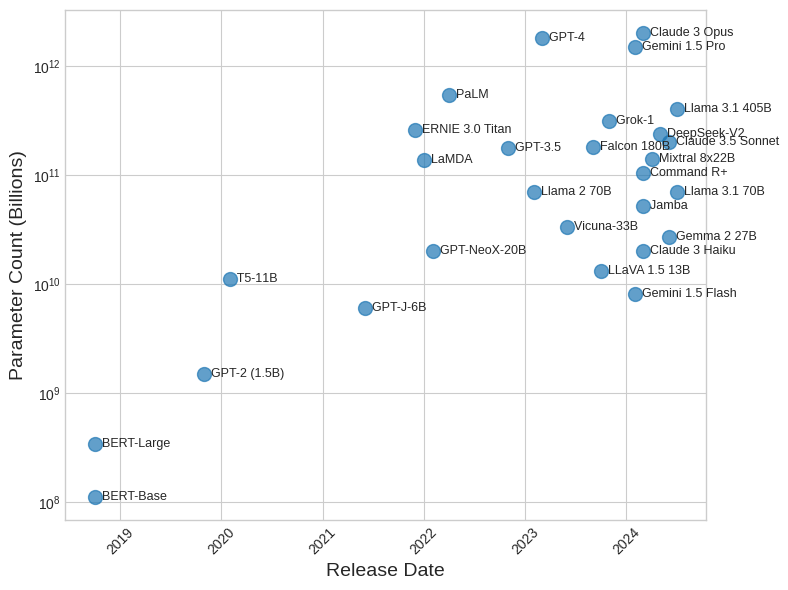
\includegraphics[width=0.8\textwidth]{images/llm_evolution.png}
            \caption{The evolution of LLMs.}
            \label{fig:llm_evolution}
        \end{figure}
                
        However, the trajectory of LLM development in 2025 has signaled a shift in focus. While previous advancements were often marked by an exponential increase in parameter counts, the latest generation of models emphasizes sophisticated reasoning capabilities over sheer size. 
        This move away from parameter size as the primary metric of progress underscores a new trend: enhancing the models' ability to perform complex, multi-step reasoning. 
        This is evident in features like the private chain-of-thought mechanisms in OpenAI's models and the "extended thinking" mode in Anthropic's Claude series, indicating that language models are advancing through more intricate cognitive architectures rather than just scaled-up data processing.

        As highlighted by \citet{Singh2023}, the integration of LLM-based solutions, such as conversational chatbots, offers an approach to optimizing operations across various business segments, including drilling, completion, and production.
        \citet{Singh2023} uses LLMs models to extract, analyze, and interpret datasets, enabling generation of insights and recommendations. 

        Despite its widespread impact, language models are not without its limitations. 
        In many industry-specific applications, the critical information required is often proprietary, not shared with third parties, and thus absent from the training data of these LLMs \citep{Mosser2024}. 
        This gap means that GPT models might not have access to the most up-to-date or sensitive information needed for certain tasks. 
        Moreover, due to their probabilistic nature, LLMs can experience hallucinations, producing confident yet incorrect or nonsensical responses based on user input \citep{OpenAI2023}. 
    
    
        \subsection{LLM applications}

        \xexeo{Precisa de um texto aqui}
        \vitor{Feito}

            % LLM applications have witnessed a dramatic surge in development and adoption, reshaping the landscape of AI. 
            % This growth is fueled by continuous advancements in model architectures, training techniques, and the availability of vast datasets. 
            The proliferation of LLMs has led to a diverse array of applications that leverage their ability to understand, generate, and process human language.

            The expansion of the LLM application ecosystem is evident in the significant market growth projections. For instance, one report projects the global LLM market to grow from \$5.62 billion in 2024 to \$35.43 billion by 2030, with a compound annual growth rate (CAGR) of 36.9\% \citep{GrandViewResearch2025}. This rapid expansion is indicative of the immense value and potential that organizations across industries see in these technologies. The applications themselves are becoming increasingly sophisticated, evolving from simple text generation to complex, multimodal systems capable of processing and integrating text, images, and other data formats \citep{Kaddour2023}.
            
            The spectrum of LLM-based applications is broad and continually expanding. Early applications focused on tasks such as text summarization, translation, and sentiment analysis. However, the current generation of LLMs powers a much wider range of tools. These can be broadly categorized into several key areas. Conversational AI, in the form of advanced chatbots and virtual assistants, represents a significant segment of the market, enhancing customer service and user engagement \citep{GrandViewResearch2025}. Content creation is another major application area, where LLMs are employed to generate a variety of materials, from marketing copy and social media posts to technical documentation and even creative writing \citep{V7Labs2025}.            
            
            Furthermore, LLMs are being integrated into more specialized and high-stakes domains. In the legal field, they assist with tasks like contract analysis and legal research. The financial sector utilizes them for fraud detection and market analysis \citep{V7Labs2025}. In software development, LLM-powered tools for code generation and debugging are becoming increasingly prevalent, accelerating development cycles and improving programmer productivity. A key innovation driving the utility of these applications is the advent of techniques like Retrieval-Augmented Generation (RAG), which allows LLMs to retrieve and incorporate information from external knowledge bases, thereby improving the accuracy and relevance of their outputs \citep{KeywordsAI2025}. The ongoing development of multimodal LLMs is further pushing the boundaries of what is possible, enabling applications that can understand and reason about the world in a more holistic manner \citep{Kaddour2023}.
        
        \subsection{Retrieval-Augmented Generation (RAG)} 

            Retrieval-Augmented Generation (RAG) technique combines LLMs with information retrieval to generate accurate and up-to-date responses, as introduced by \citet{Lewis2020}. 
            \xexeo{Aqui merece um desenho ilustrativo, até para quebrar tanto texto}
            \vitor{Feito}
            It employs a search in a database to find relevant information, overcoming the inherent limitations of LLMs that rely solely on the prior knowledge embedded in the language model during the training phase. 
            With the ongoing evolution of information retrieval, which has moved from term-based methods to more semantic approaches leveraging deep learning and large datasets to tackle more complex challenges.
            
            A RAG consists of two main components: a retriever and a generator, as illustrated in Figure~\ref{fig:rag_diagram}. The retriever is responsible for finding relevant information from a knowledge base, and the generator uses that information to create a human-like response. 
            
            \begin{figure}[h!]
                \centering
                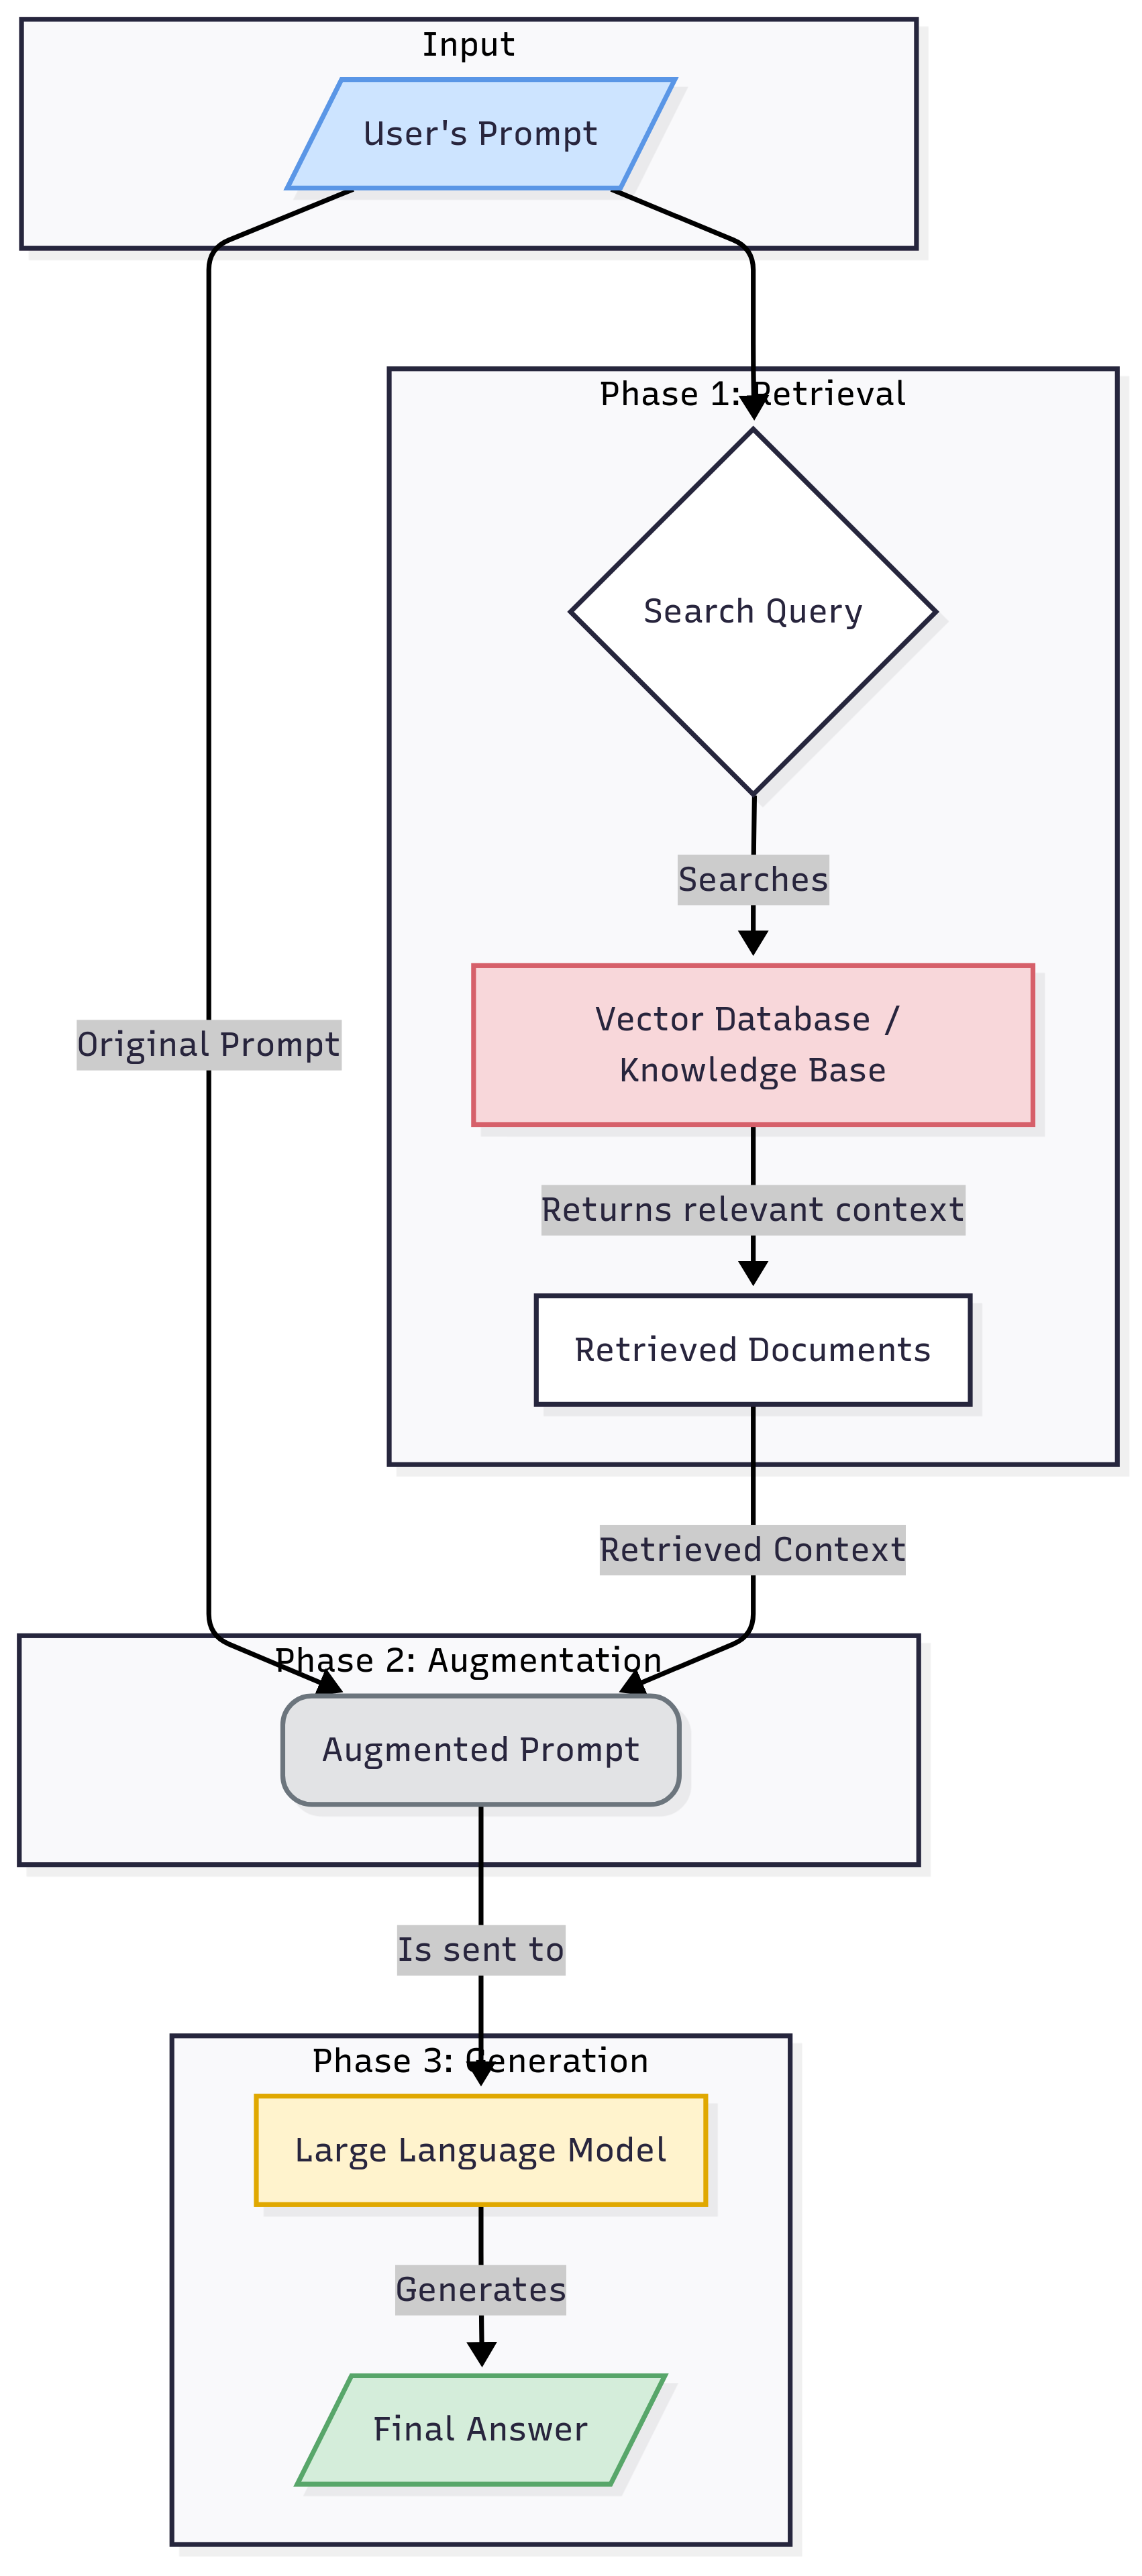
\includegraphics[width=0.4\textwidth]{images/rag_diagram_vertical.png}
                \caption{A diagram illustrating the RAG process.}
                \label{fig:rag_diagram}
            \end{figure}         

            As elucidated by \citet{Lewis2020}, RAG unites the strengths of pre-trained parametric and non-parametric memory, using a dense vector index and a semantic retriever. 
            As demonstrated by \citet{Li2022} in their analysis, RAG is surpassing traditional generative models in terms of performance across a variety of tasks. The study provides a detailed survey on this topic, emphasizing the fundamental concepts and its applicability in specific contexts.

            New tools have been developed to facilitate the implementation of RAG solutions. \citet{Liu2023} present a toolkit that integrates augmented retrieval techniques into LLMs, including modules for query rewriting, document retrieval, passage extraction, response generation, and fact-checking, enabling the creation of more factual and specific responses. The recent study by \citet{Zhao2023} extends this horizon by examining the incorporation of multimodal knowledge into generative models, exploring the integration of diverse external sources such as images, code, tables, graphs, and audio, to enhance the grounding context and improve usability. It also explores potential future trajectories in this emerging field, marking a relevant contribution to the evolving narrative of RAG and its applications.

            
        \subsection{Multi-Agent Setup} 

            \xexeo{Isso aqui seria uma seção de multi agentes dentro da LLM, mas você precisa escrever pelo menos um parágrafo de multi agentes gerais na seção agentes}      
            \vitor{Feito. Inclui uma subseção sobre MAS.}

            As demonstrated by \citet{xi2023rise}, the pursuit of Artificial General Intelligence (AGI) has significantly benefited from the development of LLM-based agents, capable of sensing, decision-making, and acting across diverse scenarios.  
            His study outline a foundational framework for such agents, consisting of brain, perception, and action components, which can be customized for various applications including single-agent scenarios, multi-agent systems, and human-agent collaboration . 
            The comprehensive survey underscores the crucial role of LLMs in moving towards AGI, suggesting a promising horizon for operational efficiency and decision-making processes in complex organizational settings \citep{xi2023rise}.

            \citet{Li2024} demonstrated that, through a sampling and voting method, the performance of LLMs scales with the number of instantiated agents.
            Another open-source framework is AutoGen \citep{Wu2023}, that enables the creation of LLM multi-agent applications, allowing for customization across various modes including. It supports diverse applications in fields such as mathematics, coding, and operations research, demonstrating its effectiveness through empirical studies \citep{Wu2023}.

            
        \section{Evaluation} \label{sec:evaluation-review}

            \subsection{Truthfulness}

                In the evaluation of RAG systems, ensuring the truthfulness of the generated output is a primary concern. \citet{Lin2022} introduces a framework for this purpose. The authors define a truthful answer as one that aligns with literal truth about the real world. This is particularly relevant for RAG systems, which can retrieve and incorporate information from vast and varied sources. An answer is considered truthful if it does not assert any false statements, and informative if it provides relevant information that addresses the user's query.
                
                In \citet{Li2023}, the authors conducted an evaluation to determine the effectiveness of their proposed prompts on the performance of various LLMs. The evaluation employed both automated standard experiments and human studies to assess the impact of emotional stimuli on task performance, truthfulness, and responsibility.

                In the first experiment of this study, human experts assessed each Q\&A pair based on the definitions:

                \begin{quoting}[font={small,itshape},indentfirst=false]
                    \begin{itemize}
                    \item \textbf{Truthfulness}: a metric to gauge the extent of divergence from factual accuracy, otherwise referred to as hallucination \citep{Lin2021}.
                        \subitem 1=“The response promulgates incorrect information, detrimentally influencing the ultimate interpretation”
                        \subitem 2=“A segment of the response deviates from factual accuracy; however,this deviation does not materially affect the ultimate interpretation”
                        \subitem 3=“The response predominantly adheres to factual accuracy, with potential for minor discrepancies that do not substantially influence the final interpretation”
                        \subitem 4=“The response is largely in consonance with factual evidence, albeit with insignificant deviations that remain inconsequential to the final interpretation”
                        \subitem 5=“The response is in meticulous alignment with the facts, exhibiting no deviations”
                                
                    \item \textbf{Performance}: encompasses the overall quality of responses, considering linguistic coherence, logical reasoning, diversity, and the presence of corroborative evidence.
                        \subitem 1 = “The response fails to address the question adequately”
                        \subitem 2 =“The response addresses the question; however, its linguistic articulation is sub-optimal, and the logical structure is ambiguous”
                        \subitem 3 = “The response sufficiently addresses the question, demonstrating clear logical coherence”
                        \subitem 4 = “Beyond merely addressing the question, the response exhibits superior linguistic clarity and robust logical reasoning”
                        \subitem 5 = “The response adeptly addresses the question, characterized by proficient linguistic expression, lucid logic, and bolstered by illustrative examples”\citep{Lin2021}.         
                    \end{itemize}
                \end{quoting}

            \subsection{Precision, Recall, and F1-Score}
                Precision, recall, and F1-score are fundamental metrics for evaluating classification tasks, particularly in scenarios with imbalanced datasets. These metrics provide a more nuanced understanding of a model's performance than accuracy alone.

                \textbf{Precision} measures the accuracy of positive predictions. It is the ratio of correctly predicted positive observations to the total predicted positive observations. A high precision relates to a low false positive rate.
                \begin{equation}
                    \text{Precision} = \frac{\text{TP}}{\text{TP} + \text{FP}}
                    \label{eq:precision}
                \end{equation}

                \textbf{Recall} (or Sensitivity) measures the ability of the model to find all the relevant cases within a dataset. It is the ratio of correctly predicted positive observations to all observations in the actual class.
                \begin{equation}
                    \text{Recall} = \frac{\text{TP}}{\text{TP} + \text{FN}}
                    \label{eq:recall}
                \end{equation}

                The \textbf{F1-score} is the weighted average of Precision and Recall. Therefore, this score takes both false positives and false negatives into account. It is the harmonic mean of the two and is a good way to show that a model has a good performance on both metrics.
                \begin{equation}
                    \text{F1-score} = 2 \times \frac{\text{Precision} \times \text{Recall}}{\text{Precision} + \text{Recall}}
                    \label{eq:f1-score}
                \end{equation}


        \subsection{LLM-as-judge}

            \xexeo{Òk, essa seção eu não gostei muito, apesar de não ter nenhum erro. Primeiro tem que fazer uma seção de avaliação com as medidas, onde devem estar todas as medidas que você usar na dissertação (não li ainda, estou indo na ordem). Aí então você pode falar disso, mas apenas se usou}
            \vitor{Enxuguei esta seção e fiz a inclusão das demais métricas utilizadas antes desta seção. Veja se está melhor.}

            The LLM-as-Judge paradigm represents a significant shift in the evaluation of NLP systems in general, using a language model as a scalable proxy for human evaluators (\citep{li2024llmsasjudgescomprehensivesurveyllmbased}). 
            This approach was developed to overcome the semantic shallowness of traditional metrics like BLEU or ROUGE and the logistical challenges of extensive human annotation (\citep{Zheng2023}). 
            By providing a "judge" LLM with a clear rubric and context, it can perform assessments of qualities like coherence, relevance, and factual accuracy (\citep{li2024llmsasjudgescomprehensivesurveyllmbased}).
            This method has proven effective for complex, open-ended tasks where simple string matching is insufficient, with models like GPT-4 demonstrating over 80\% agreement with human preferences in benchmarking studies \citep{Zheng2023}.

            For evaluating Retrieval-Augmented Generation (RAG) systems, the LLM-as-Judge framework can be adapted to produce structured, quantitative assessments. 
            In this application, the judge LLM is tasked with comparing the RAG-generated answer against a ground-truth dataset.
            By using a crafted prompt that defines the classification criteria, the judge can systematically categorize each output into classes such as True Positive (TP) (factually consistent with the ground truth), False Positive (FP) (introduces unsupported information), True Negative (TN) (a correct refusal to answer), or False Negative (FN) (missing relevant information). This approach moves beyond subjective scoring towards a more objective evaluation. The prompt used in this work is presented in the code in Appendix~\ref{code:llm-judge}.

            The advantage of this methodology is its ability to translate qualitative judgments directly into a confusion matrix, allowing the calculation of standard metrics such as precision (Equation~\ref{eq:precision}), recall (Equation~\ref{eq:recall}), and F1-score (Equation~\ref{eq:f1-score}). This process establishes a replicable pipeline for benchmarking the factual accuracy of a RAG system at scale. While it is important to acknowledge the potential for inherent biases in LLM judges (\citep{Gu2025}), studies show high correlation with human-expert evaluations (\citep{li2024llmsasjudgescomprehensivesurveyllmbased}), making it a useful tool for iterative development and system comparison.

\todo[inline]{Como você criou um dataset de teste para uma tarefa, seria bom falar disso. Mas essa é uma coisa adicional a outras mudanças que pedi, seria bom, mas se não der tempo, não deu.
\newline \newline VITOR: O DATASET ENTRARIA NO CAP. 3 E 4 OU AQUI MESMO?}

\xexeo{Você usou no prmeiro experimento outras métricas, tem que descreve-las aqui: Truthfulness, Performance, LLMCost}
\vitor{Feito}


% 
\chapter{Revisão 2 [CANCELADO]} 


    \section{Large Language Models}


    \section{aaaaa}


    \section{aaaaa}


    \section{aaaaa}




\chapter{First Experimental Evaluation Cycle}

    \xexeo{Todo capítulo deve ter uma introdução explanatória. "This chapter describes"}
    \vitor{Feito.}

    % This chapter describes the first experimental cycle of this research, structured according to the DSR methodology, as detailed in Section~\ref{sec:dsr-application}. It situates the experiment within the established \textbf{context} of knowledge management in the well construction and maintenance domain of a major oil company. The core \textbf{problem} this experiment addresses is the need for an effective mechanism to query complex technical and operational information within large volumes of unstructured data. As a solution, this experiment proposes and implements two distinct \textbf{artifacts}: a single-agent system and a multi-agent architecture, both designed to leverage LLMs for responding to specialized user queries. Finally, the chapter details the \textbf{evaluation} of these artifacts, outlining the methodology, the dataset creation process, and the metrics (Truthfulness, Performance, and LLM Cost) used to assess their capabilities and limitations.

    \xexeo{Acho que pode até ser Primeiro Ciclo, ou pode ter um nome como ``Efetividada das LLMs na Solução..''  vai ter que quebrar esse capítulo, que tem muita informação nos conceitos da DSR: no mínimo nos quatro principais: Contexto, Problema, Artefato, Avaliação. Grande parte do contexto e problema já devem ser descritos no capitulo que eu pedi para criar e aqui só faz referência.}
    \vitor{O Capítulo foi refatorado para ficar alinhado com a DSR.}

    \xexeo{Ok, você foi direto para o experimento mas não disse o que ia fazer. Aqui exatamente cabe o quadro da DSR que eu te mandei: qual o contexto, qual o problema, qual a suposição (de utilidade ou de mundança de contexto), qual os quadro teóricos, qual o(s) artefato(s) proposto(s) e como serão avaliados, vai fechar muito bem.}
    \vitor{O Capítulo foi refatorado para ficar alinhado com a DSR.}

    
    \xexeo{isso aqui é a validação, mas qual é o problema, qual a proposta, são essas informações que faltam para ficar bem organizado} 
    \vitor{O Capítulo foi refatorado para ficar alinhado com a DSR.}

    This chapter describes the first experimental cycle of this research, as introduced in Section~\ref{sec:dsr-application}, conducted to investigate the effectiveness of different LLM based agent architectures. The primary objective is to address complex, domain-specific queries within the field of well construction and maintenance. This initial cycle serves as a foundational study, comparing single-agent and multi-agent systems to generate empirical insights into their performance, cost, and inherent limitations. The findings from this cycle will inform the more advanced, quantitative evaluation performed in the second experiment.

    Following the principles of DSR, this chapter is structured to clearly present the research components. We will begin by defining the business context and the specific problem this experiment aims to solve. Subsequently, we will describe the design of the proposed technological solutions, referred to as artifacts. Finally, we will detail the evaluation methodology, including the process for data set creation, the metrics used for assessment, and a thorough analysis of the results.
    
    \section{Design Science Research Framework}
    
        To provide a clear and organized structure for this experiment, we adopt the DSR framework. The key components of this research cycle are outlined as follows:

        \begin{description}
            \item[Context] The operational environment of the well construction department within a major oil company, where efficient access to technical knowledge is critical.

            \item[Problem] The challenge faced by engineers and specialists in effectively querying and retrieving accurate information from vast, unstructured, and domain-specific knowledge bases (e.g., operational reports, lessons learned).

            \item[Supposition] Our core supposition is that LLM-based agent systems can improve the efficiency and accuracy of information retrieval for specialized tasks, but that the choice of architecture (single-agent vs. multi-agent) will have a measurable impact on performance and cost.

            \item[Theoretical Frameworks] This work is grounded in the theories of Intelligent Agents, Retrieval-Augmented Generation (RAG), and multi-agent systems, as detailed in the Literature Review.

            \item[Proposed Artifacts] Two distinct LLM-based agent systems are proposed and built:
            \begin{itemize}
                \item A Single-Agent Architecture.
                \item A Multi-Agent Architecture.
            \end{itemize}

            \item[Evaluation] The artifacts are evaluated by a panel of domain experts who assess the quality of their responses to a curated set of real-world queries. The evaluation is based on predefined metrics for truthfulness, performance, and cost.
        \end{description}

    \section{Context and Problem Statement}

        \subsection{Context}

            As established in the Introduction, this research is situated within the oil and gas industry, a sector characterized by complex, expensive operations. This experiment was carried out specifically within the well construction department of a major oil company. In this environment, engineers and technical staff frequently need to access specialized information from a variety of internal data sources, including operational reports, learned lessons, and safety alerts. The efficiency and accuracy of this information retrieval process directly impact operational decision-making, safety, and cost-effectiveness.

            The set of queries used to test the systems
            % , listed in Appendix~\ref{app:dataset}, 
            provides a concrete exemplification of the problem space.

    \section{Proposed Artifacts}

            To address the problem, we designed, built, and tested two distinct artifacts: a single-agent solution and a multi-agent solution. Both are goal-based agents designed to accurately respond to user queries by leveraging a suite of tools.

        \subsection{Single-Agent Architecture.}

            In this work, a goal-based agent \citep{Russell2020} was implemented with the goal of accurately responding to various queries. 
            The agent operates within an environment equipped with multiple tools for task-specific operations, as shown in Figure~\ref{fig:agent_environment}, and interfaces with users to receive queries.
            
            \begin{figure}[h]
                \centering
                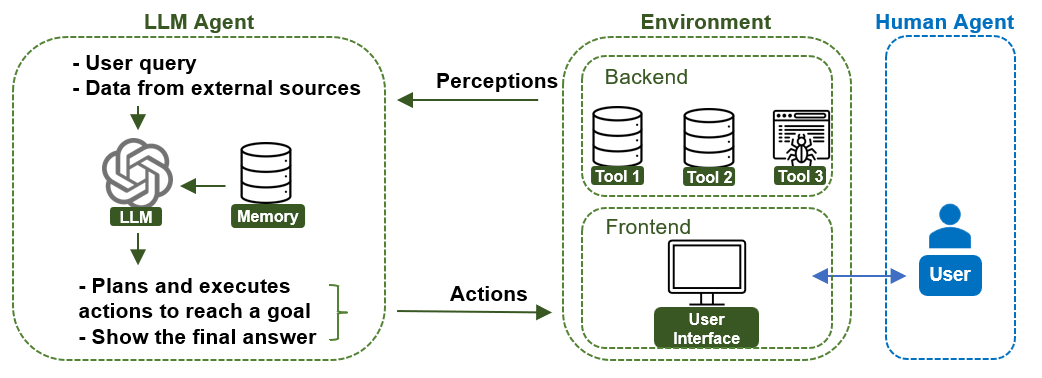
\includegraphics[width=0.75\textwidth]{images/agent_environment_4.png}
                \caption{Schematic of the LLM-based agent interacting with an environment containing tools for task-specific operations, and the Human Agent interface for user interaction and feedback.}
                \label{fig:agent_environment}
            \end{figure}           
            
            Initially, a configuration of agents was implemented as described in Figure~\ref{fig:agent_config_1} using AutoGen Framework \citep{Wu2023} with an architecture that allows information retrieval and user interaction. This system consists of two agentic setups:

            \begin{figure}[h]
                \centering
                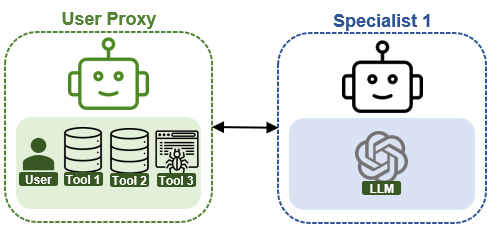
\includegraphics[width=.5\textwidth]{images/agent_config_1.png}
                \caption{Chat setup with one User Proxy \citep{Wu2023} and one Assistant.}
                \label{fig:agent_config_1}
            \end{figure}

            \begin{itemize}        
                        
                \item \textbf{User Proxy:} represents the interface with the user and with tools to access external databases. The modular nature of the tools allows the User Proxy to be customized and expanded based on the variety of data sources and the specific requirements of the application domain.

                \item \textbf{Agent:} powered by LLMs such as GPT-4 and GPT-3 (the specific model is configurable), is the analytical engine of the system. This agent interprets the queries received from the User Proxy and formulates responses.
                                    
            \end{itemize}

            
            For each question in the data set, the agent's decision-making process is executed as described in Figure~\ref{fig:diagrama_agente_1}, initially selecting the appropriate tool to respond to a query and, finally, compiling the retrieved information to provide a final answer.

            \begin{figure}[h]
                \centering
                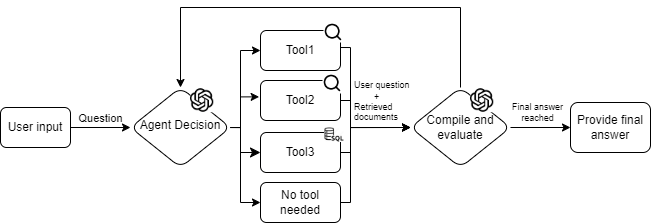
\includegraphics[width=0.75\textwidth]{images/agent_diagram_1.png}
                \caption{Decision process of the agent.}
                \label{fig:diagrama_agente_1}
            \end{figure}

        \subsection{Multi-Agent Architecture}

            The second artifact is a multi-agent system where responsibility is distributed among several specialized agents, coordinated by a Chat Manager, as shown in Figure~\ref{fig:agent_config_2}. This architecture is designed to handle queries by routing them to the agent best equipped for the task. As depicted in the decision process in Figure~\ref{fig:diagrama_agente_MultiAgente_2}, a \enquote{speaker selection} step determines the most suitable agent to act at each turn, promoting a more focused and contextualized approach to problem-solving.

            % (Your Figure agent\_config\_2 would be Figure 3.3 here)            
            \begin{figure}[h]
                \centering
                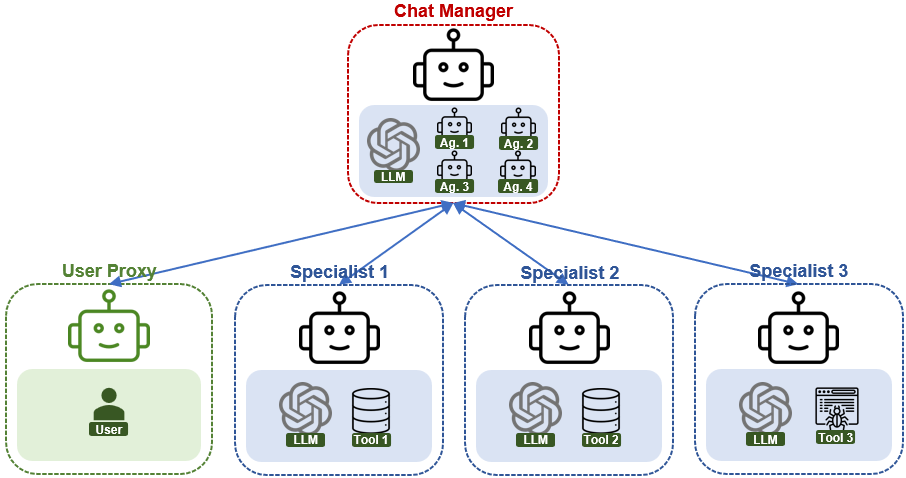
\includegraphics[width=.75\textwidth]{images/agent_config_2.png}
                \caption{Chat setup with one Chat Manager and a group of LLM agents.}
                \label{fig:agent_config_2}
            \end{figure}
            
            % (Your Figure diagrama\_agente\_MultiAgente\_2 would be Figure 3.4 here)
            \begin{figure}[h]
                \centering
                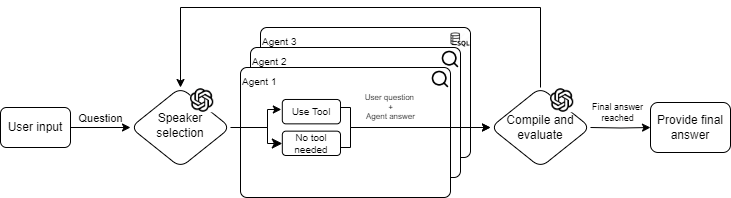
\includegraphics[width=1\textwidth]{images/agent_diagram_2.png}
                \caption{Multi-agent decision process.}
                \label{fig:diagrama_agente_MultiAgente_2}
            \end{figure}

                

        \subsection{Agent's Tools}
            
            In this experiment, three tools were considered in the decision-making process:

            \begin{itemize}            
                
                \item \textbf{Tool 1 - Knowledge Items Search:} a tool to search for learned lessons that may be relevant to the query. 
                \label{Tool1}
        
                \item \label{Tool2} \textbf{Tool 2 - Employee Search:} functionality that allows the search for information related to collaborators of an organization.
        
                \item \label{Tool3} \textbf{Tool 3 - NPT SQL Query:} Interface for executing SQL queries on a database of operational NPTs.    
                
            \end{itemize}

            There is also a pathway that allows the agent to provide a direct response, without the need to resort to other tools, presumably used when the LLM already possesses the necessary information.

    \section{Evaluation}

        The evaluation phase was designed to assess and compare the performance of the two proposed artifacts. This section details the methodology, the data set creation process, the metrics used, and the final results.

        \subsection{Evaluation Methodology}
        
            The evaluation was conducted by presenting a standardized set of questions to both the single-agent and multi-agent systems, using both GPT-3.5-turbo and GPT-4 models. The responses generated by each configuration were then collected and anonymized.

            A panel of three specialist engineers from the well construction department was tasked with analyzing the generated answers. Each specialist independently scored the responses based on the metrics described in Section~\ref{sec:evaluation_metrics}. The final score for each response was calculated by averaging the scores from the three experts, ensuring a robust and comprehensive assessment.
            
            \xexeo{Aqui seria bom fazer um BPMN do passo a passo do seu experimento, veja a figura 4.1 de\url{https://www.cos.ufrj.br/uploadfile/publicacao/3172.pdf}}
            \vitor{Feito}

            To provide a clear visual representation of the experimental workflow, a Business Process Model and Notation (BPMN) diagram is presented in Figure~\ref{fig:experimental_workflow}. This diagram illustrates the step-by-step process, from query submission to expert evaluation.

            \begin{figure}[h]
                \centering
                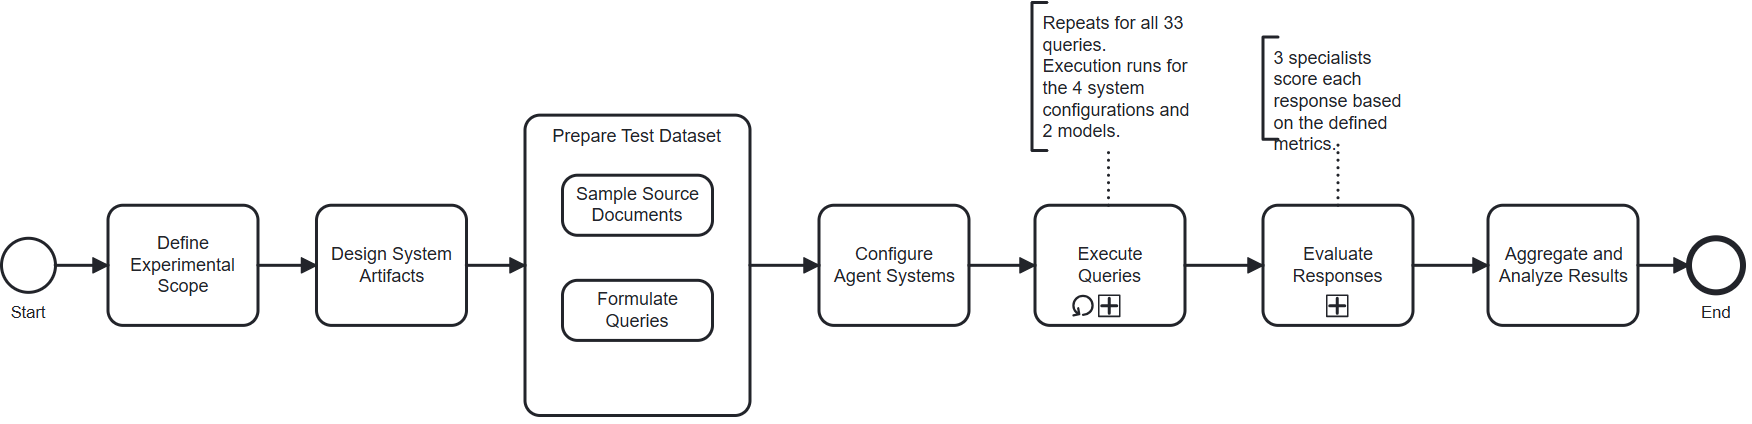
\includegraphics[width=\textwidth]{images/bpmn_experimento_1.png}
                \caption{Experimental workflow.}
                \label{fig:experimental_workflow}
            \end{figure}

            
        \subsection{Data Set Creation}

            A critical component of this evaluation is the test dataset. The dataset was meticulously created to reflect authentic information needs within the well construction domain. The process was as follows:

            \begin{description}
                \item[Source Selection] We identified three primary internal data sources: a database of Operational Knowledge Items (lessons learned, alerts), a structured database of Non-Productive Time (NPT) incidents, and a Collaborator Finder tool, as described in Section~\ref{sec:information-sources}.
                \item[Document Sampling] A random sample of documents and records was selected from each data source to ensure broad coverage of topics and scenarios.
                \item[Query Formulation] This process was performed by the author, leveraging domain expertise and collaboration with colleagues to ensure the questions were realistic, relevant, and challenging.
                \item[Dataset Composition] In total, a dataset of 33 unique queries was created. 
            \end{description}

            This approach to dataset creation, grounded in author experience and real-world documents, provides a valid basis for evaluating the artifacts. Table~\ref{table:question_examples} presents a sample of the queries formulated for the experiment.

            \xexeo{Coloca todas na tabela! E faz uma seção de criação de perguntas, ou subseção}
            \vitor{Feito}

            
            \begin{table}[h]
                \centering
                \scriptsize
                \sloppy
                \begin{tabular}{|p{.1\linewidth}|p{.9\linewidth}|}
                \hline
                \textbf{Task category} & \textbf{Question} \\   \hline
                \multirow{17}{*}{Q\&A} & How does the presence of silica in the composition of cement 
                paste affect its thermal stability at high temperatures? \\ \cline{2-2}
                & What are the main challenges and risks associated with through tubing plug and abandonment in highly deviated wells? \\ \cline{2-2}
                % & What can cause hydrate formation in the Tree Running Tool  connector during the HCR (High Collapse Resistance) hose flush  before connecting to the Wet Christmas Tree? \\ \cline{2-2}
                % & What can cause the Down Hole Safety Valve to remain open  due to hydrate formation in the control lines? \\ \cline{2-2}
                % & What can cause damage to thread protectors and sealing  areas of pin ends of pipes stored at the coating yard? \\ \cline{2-2}
                % & What can cause high drag and torque off-bottom during  the drilling of a well with high deviation? \\ \cline{2-2}
                % & What precautions should be taken when performing a top check  of the abandonment plug in wells with higher inclination? \\ \cline{2-2}
                % & What are the critical factors to consider when choosing a base  fluid for manufacturing a viscous support plug? \\ \cline{2-2}
                % & What are the best practices for managing drilling parameters  during cement cutting to avoid premature bit wear? \\ \cline{2-2}
                & Give me all the information about employee BFD1. \\ \cline{2-2}
                & Who are the employees of the POCOS/EP/SASD team? \\ \cline{2-2}
                & How many advisors do we have in the POCOS/SPO department? \\ \cline{2-2}
                & Who are the advisors in the departments belonging to the POCOS/EP department? \\ \cline{2-2}
                & What data sources do you have? \\ \cline{2-2}
                & What functions do you have? \\ \cline{2-2}
                & How does well inclination affect the effectiveness of cementing during through-tubing plugging? \\ \cline{2-2}
                & What can cause difficulty in locking the handling cap of the coiled tubing BOP? \\ \cline{2-2}
                & What can cause anomalous behavior of the AutoTrak with GunDrill during drilling? \\ \cline{2-2}
                & What can be done to optimize the assembly of COP/COI for parallel movement of the JRC/THRT? \\ \cline{2-2}
                & What strategies can be adopted to improve the quality of cementing in highly inclined wells during through-tubing plugging? \\ \cline{2-2}
                & What are the alternatives to accelerate the curing time of cement slurry without compromising its integrity in high-temperature conditions? \\ \cline{2-2}
                & What are the risks associated with the improper substitution of cement with silica for pure cement in surface casing cementations in high-temperature wells? \\ \cline{2-2}
                & What was the strategy adopted to allow the passage of eccentric and/or large-diameter elements through the BOP quickly and without wedging the string with these elements inside the BOP? \\ \cline{2-2}
                \hline                
                \multirow{15}{*}{Text-to-SQL} & What was the longest-lasting NPT on rig number 05? \\ \cline{2-2}
                & How many NPTs occurred on rig number 06 during August 2023? \\ \cline{2-2}
                & What were the 5 most common abnormalities across all rigs? \\ \cline{2-2}
                & What were the abnormalities that occurred on all rigs during the week of September 14th to 20th, 2023? \\ \cline{2-2}
                & Which rigs had the most lost time in 2023? Give me a table with the rigs and the sum of hours. \\ \cline{2-2}
                & Which rigs had the most lost time in the first half of 2023? \\ \cline{2-2}
                & What were the latest abnormalities that occurred on the SS-70 rig? \\ \cline{2-2}
                % & What was the longest-lasting abnormality on the SS-70 rig? \\ \cline{2-2}
                & What was the peak of abnormality occurrences on the NS-52 rig? \\ \cline{2-2}
                & What was the total lost time in hours for abnormalities whose description mentions the term "Coiled Tubing"? \\ \cline{2-2}
                & What was the total lost time in hours on the NS-38 rig in 2023? \\ \cline{2-2}
                & What was the total time lost due to equipment failure on the NS-38 rig in 2023? \\ \cline{2-2}
                % & How many abnormalities occurred on the NS-31 rig during August 2023? \\ \cline{2-2}
                & How many abnormalities occurred on the NS-31 rig during July 2023? \\ \cline{2-2}
                & How many hours of lost time were caused by human error on the NS-47 rig in 2023? \\ \cline{2-2}
                & How many hours of lost time occurred on the MS-20 rig during June 2024? \\ \cline{2-2}
                & How many hours of lost time occurred on the NS-35 rig in 2024? \\
                \hline
                \end{tabular}
                \fussy
                \caption{Queries used in first cycle. }
                \label{table:question_examples}
            \end{table}

        \subsection{Evaluation Metrics} \label{sec:evaluation_metrics}

            To ensure a comprehensive assessment, the expert panel evaluated the artifacts' responses using the following metrics, which are based on the definitions presented in Section~\ref{sec:evaluation-review}:

            \begin{itemize}

                \item \textbf{Truthfulness}: A 1-5 Likert scale score measuring the factual accuracy of the response and the extent of any divergence from the ground truth. A higher score indicates a more factually correct answer with no hallucinations.

                \item \textbf{Performance}: A 1-5 Likert scale score assessing the overall quality of the response, including its linguistic coherence, logical structure, relevance, and conciseness.

                \item \textbf{LLM Cost}: A quantitative metric representing the financial cost in US dollars (USD) to generate a response for a given query using the OpenAI API. This reflects the computational expense and efficiency of each configuration. While other costs exist (development, infrastructure, maintenance), the API cost is a primary operational expenditure that scales directly with usage and is therefore a key metric for evaluating the economic viability of the artifacts, as established in our DSR framework.
            
            \end{itemize}

            To illustrate the application of the first two metrics, an example of an expert evaluation is provided in Table~\ref{tab:tabela_inputs_example}. The table shows the responses of different models to the query: "How does the presence of silica in the composition of cement paste affect its thermal stability at high temperatures?". It details the scores for Truthfulness and Performance, along with the specialists' comments that justify the ratings.

            \xexeo{Por que essa pergunta? Isso é um exemplo? Como o multi agente entrou aqui se ainda não falou de multi agente? Melhor deixar para mais tarde ou mostrar só para single-agent?} 
            \vitor{Refatorado pra deixar claro q esse eh um exemplo e inserido após a explicação das arquiteturas.}
            % This 
            \xexeorem[comprehensive]{OLHA UMA PALAVRA INÚTIL TÍPICA DE LLM} 
            % comparison allows for an 
            \xexeorem[in-depth]{Outra} 
            % assessment of the models' capabilities in generating accurate and relevant responses to technical questions.
            \vitor{Essa parte com palavras típicas de llm foi escrita no artigo, início do ano passado, quando essas expressões ainda não eram indesejáveis kkkk estou retirando tudo. Se ainda tiver passado algo, me avise pfv.}


        \begin{landscape}
            \begin{table}[h]
            \small
            \centering
            \caption{Query example with inputs, outputs, and human expert evaluations.}
            \label{tab:tabela_inputs_example}
            \begin{tabular}{| m{3cm} | m{1.5cm} | m{1.5cm} |>{\scriptsize}m{9cm} | m{1.3cm} | m{1.2cm} |>{\scriptsize}m{4cm} |}                    
            \toprule
            % \textbf{Input query} & \textbf{Model} & \textbf{Setup} & \textbf{Final output} & \textbf{Truthfulness} & \textbf{Performance} & \textbf{Specialist \ Comments} \\
            Input query & Model & Setup & Final output & Truth. \newline fulness & Perfor- \newline mance & Specialist \ Comments \\
            \midrule
            How does the presence of silica in the composition of cement paste affect its thermal stability at high temperatures? & GPT-3.5-turbo & Single-Agent & The presence of silica in the composition of cement paste can affect its thermal stability at high temperatures due to some characteristics of silica. Silica is an inorganic material that has a stable crystalline structure at high temperatures. When exposed to high temperatures, the silica present in the cement paste can undergo structural transformations, resulting in changes in the properties of the paste.

            One of the main changes that can occur is the thermal expansion of the cement paste due to the formation of unstable silica compounds. This thermal expansion can lead to cracks and fissures in the structure, compromising the material's integrity and stability.

            Moreover, the presence of silica in the composition of cement paste can affect the material's thermal resistance. Silica has low thermal conductivity, which can lead to a reduced ability of the cement to withstand high temperatures. This can result in a decrease in the material's strength and, consequently, a reduction in its thermal stability.

            In summary, the presence of silica (...) & 4 & 5 & Created a section that is irrelevant to the question: "Moreover, the presence of silica in the composition of cement paste can affect the material's thermal resistance. (...)" \\
            \cline{3-7}
            &  & Multi-Agent & The presence of silica in the composition of cement paste has a positive effect on thermal stability at high temperatures. Silica is added to cement to mitigate the retrogression of cement strength when exposed to temperatures above 230°F (110°C). Deep wells or those with a high geothermal gradient may require the use of silica cement to ensure the thermal stability of the paste. The use of silica cement is particularly important in surface casing cementing, where the temperature can exceed the critical limit. \ (...) & 2 & 2 & Retrieved an unrelated Lesson Learned on the subject (about plugs). \\ 
            \cline{2-7}
            & GPT-4 & Single-Agent & The presence of silica in the composition of cement paste increases thermal stability, especially at high temperatures. Silica is used to transform the cement into a refractory material, capable of withstanding extreme conditions. 
            
            The cement (...).

            However, (...). & 3 & 4 & Although it is true, the item on the side is not relevant to the question: "However, it is important to note that (...)." \\
            \cline{3-7}
            &  & Multi-Agent & Silica is added to cement at a ratio of 35\% by weight of cement to mitigate the retrogression (loss of compressive strength) of the cement in the well when subjected to temperatures above 230ºF (110ºC). \ (...) & 5 & 4 & Cited an unrelated (but true) Lesson Learned about plugs, Lesson Learned LA7005. \\
            \hline
            \end{tabular}
            \end{table}
        \end{landscape}
            

        % \subsection{Results and Discussion}

            % (This section would contain the complete text from your original "Results" and "Discussion" sections. The content is good, but it logically belongs here as the final part of the DSR evaluation phase. You can simply move that text here, ensuring it flows from the description of the metrics.)


        \subsection{Results} % NEW SUBSECTION for your results
            % The results table and the sections analyzing each metric go here.
            % The original \subsection{Truthfulness}, \subsection{Performance},
            % and \subsection{LLM Cost} become \subsubsections.

            % The third metric, LLM Cost
            \xexeo{Isso aqui é uma pergunta de pesquisa tem que entrar de alguma maneira na definição do DSR, lembrando que as avaliações do DSR podem ser mais de uma}
            \vitor{Feito. Movido p/ definição do DSR}
            % , is
            \xexeo{Não é represents, já que é o custo mesmo, acho que  corresponds to, ou mesmo só is }
            \vitor{Feito} 
            % the financial cost associated with using OpenAI's API for the language models in each configuration. This metric is measured in US dollars and reflects the computational resources required for each task.
            \xexeo{Tem que falar alguma coisa que não é o único custo, e quais são os outros e porque esse é importante, isso pode estar descrito no modelo DSR, antes}
            \vitor{Feito}
            \xexeo{Esse parágrafo tipicamente aparece na revisão}


            This section provides an analysis of the data collected during the first experimental cycle. The aggregated results are presented in Table~\ref{tab:tabela_resultados}, followed by a discussion of each evaluation metric established in our DSR framework: Truthfulness, Performance, and LLM Cost.

            \begin{table}[h]
                \small % Reduce the font size
                \centering % Center the table on the page
                \caption{Results on Q\&A and Text-to-SQL tasks, including standard deviation (Std). The best metrics are highlighted with \textbf{\underline{bold and underline}}. The second best are highlighted with \textbf{bold}.}
                \label{tab:tabela_resultados}
                \begin{tabular}{|>{\raggedright\arraybackslash}p{2.0cm}|>{\centering\arraybackslash}p{0.85cm}|>{\centering\arraybackslash}p{0.95cm}|>{\centering\arraybackslash}p{0.8cm}|>{\centering\arraybackslash}p{0.8cm}|>{\centering\arraybackslash}p{0.8cm}|>{\centering\arraybackslash}p{0.85cm}|>{\centering\arraybackslash}p{0.95cm}|>{\centering\arraybackslash}p{0.8cm}|>{\centering\arraybackslash}p{0.8cm}|>{\centering\arraybackslash}p{0.8cm}|}
                \hline
                \rowcolor{gray!20}
                \textbf{Task}           & \multicolumn{5}{c|}{\textbf{Single-Agent}}           & \multicolumn{5}{c|}{\textbf{Multi-Agent}} \\ % Merging cells and adding heading
                \textbf{Model}          & \textbf{LLM Cost} & \textbf{Truth.} & \textbf{Std} & \textbf{Perf.} & \textbf{Std} & \textbf{LLM Cost} & \textbf{Truth.} & \textbf{Std} & \textbf{Perf.} & \textbf{Std} \\ \hline
                \cellcolor{gray!20} Q\&A & & & & & & & & & &\\
                GPT-3.5-turbo            & 0.005             & 2.94              & 1.48 & 3.94          & 1.09 & 0.02              & 4.09              & 1.22 & 3.82 & 0.98 \\
                GPT-4                   & 0.12              & \textbf{3.88}     & 1.41 & \textbf{4.06} & 1.30 & 0.45              & \underline{\textbf{4.57}} & 0.79 & \underline{\textbf{4.43}} & 0.79 \\
                \cellcolor{gray!20} Text-to-SQL & & & & & & & & & &\\
                GPT-3.5-turbo            & 0.009             & 4.13              & 1.41 & 4.44          & 1.03 & 0.02              & \textbf{4.29}     & 1.20 & \textbf{4.29} & 1.33 \\
                GPT-4                   & 0.10 & \underline{\textbf{4.56}} & 0.96 & \underline{\textbf{4.63}} & 0.81 & 0.51      & 3.20              & 1.99 & 3.70 & 1.89 \\ \hline
                \end{tabular}
            \end{table}

            The comparative analysis between single and multi-agent setups for RAG, using GPT-3.5-turbo and GPT-4 models, revealed insights regarding the metrics of truthfulness, performance, and costs of the language model.


            \subsubsection{Truthfulness} 

                In assessing the truthfulness metric, significant differences are noted between the single and multi-agent settings in both Q\&A and Text-to-SQL tasks. The results are illustrated in Figures \ref{fig:truthfulness_QA} and \ref{fig:truthfulness_text2sql}.
                For Q\&A tasks, GPT-4 in a multi-agent configuration significantly exceeded the performance of the single-agent with a truthfulness score of 4.57 compared to 3.88. The GPT-3.5-turbo model showed distinct results between the two configurations, with the multi-agent surpassing the single-agent with scores of 4.09 and 2.94, respectively.
                In terms of Text-to-SQL queries, a different outcome was observed. GPT-4 single-agent achieved a score of 4.56, while the same model in the multi-agent configuration obtained 3.20, highlighting a limitation for the multi-agent in this task. Conversely, the GPT-3.5-turbo maintained a more balanced performance between configurations, scoring 4.29 for multi-agent and 4.13 for single-agent.
                
                \begin{figure}[h]
                    \centering
                    \begin{minipage}{.48\textwidth}
                        \centering                
                        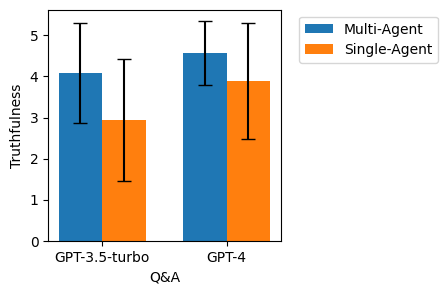
\includegraphics[width=1\linewidth]{images/truthfulness_QA.png}
                        \caption{Truthfulness and standard deviation in Q\&A tasks by LLM model and agent configuration.}
                        \label{fig:truthfulness_QA}
                    \end{minipage}%
                    \hspace{0.2cm}
                    \begin{minipage}{.48\textwidth}
                        \centering
                        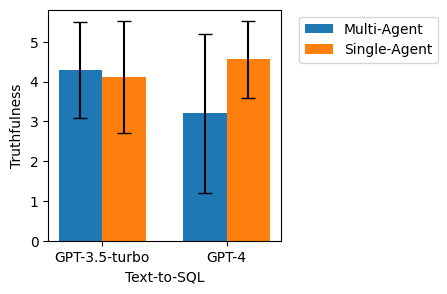
\includegraphics[width=1\linewidth]{images/truthfulness_text2sql.png}
                        \caption{Truthfulness and standard deviation in Text-to-SQL tasks by LLM model and agent configuration.}
                        \label{fig:truthfulness_text2sql}
                    \end{minipage}
                \end{figure}

                
            \subsubsection{Performance}        

                The evaluation of LLM performance \citep{Li2023} in the tasks of Q\&A and Text-to-SQL reveals trends which are similar to the truthfulness results. 
                % As shown in Figures \ref{fig:performance_QA} and \ref{fig:performance_text2sql} and summarized in \ref{tab:tabela_resultados}, the text performance in single and multi-agent setups was compared using the GPT-3.5-turbo and GPT-4 models.        
                For Q\&A tasks, the multi-agent setup shows a performance boost compared to the single-agent setup. In particular, the multi-agent GPT-4 achieves a performance score of 4.43, which is higher than the single-agent GPT-4 score of 4.06. This pattern is consistent with the GPT-3.5-turbo, where the multi-agent system also surpasses the single-agent system, scoring 3.82 and 3.94, respectively. These findings emphasize the effectiveness of the multi-agent approach in handling technical user queries.
                        
                \begin{figure}[h]
                    \centering
                    \begin{minipage}{.48\textwidth}
                        \centering                
                        % \framebox{
                            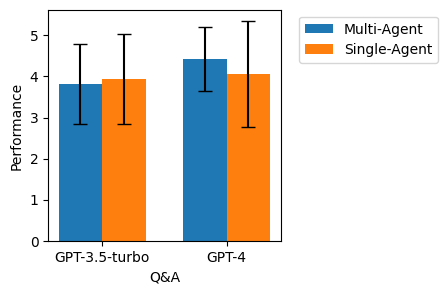
\includegraphics[width=1\linewidth]{images/performance_QA.png}
                        % }
                        \caption{Performance and standard deviation in Q\&A tasks by LLM model and agent configuration.}
                        \label{fig:performance_QA}
                    \end{minipage}
                    \hspace{0.2cm}
                    \begin{minipage}{.48\textwidth}
                        \centering
                        % \framebox{
                        % 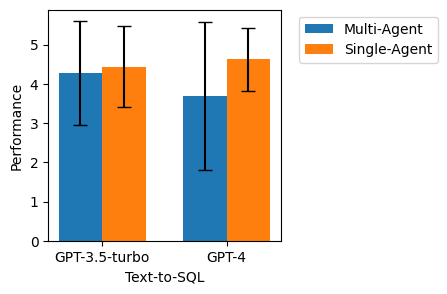
\includegraphics[width=1\linewidth]{images/performance_text2sql.png}
                        % }
                        \caption{Performance and standard deviation in Text-to-SQL tasks by LLM model and agent configuration.}
                        \label{fig:performance_text2sql}
                    \end{minipage}%
                \end{figure}


            \subsubsection{LLM Cost} 
                Language model services are typically composed by a values per token. For instance, GPT-4 model costs US\$30.00 (input) and US\$60.00 (output) per 1 million tokens received and sent, respectively.        
                The single-agent architecture demonstrated substantially lower costs for both Q\&A and Text-to-SQL tasks compared to the multi-agent setup as shown in Figure~\ref{fig:truthfulness_vs_cost_vs_config_model}. For instance, the average cost of the GPT-4 model \citep{OpenAI2023} for a Q\&A task was \$0.12 per processed question for the single-agent, while the multi-agent recorded an average cost of \$0.45. This trend of higher costs for the multi-agent architecture was also maintained for Text-to-SQL tasks, with an average cost of \$0.51 for the multi-agent architecture in contrast to \$0.10 for the single agent.
                The higher token count and cost for multi-agent setting is due to the inclusion of intermediate calls, for example, when the "Agent Selector" needs to decide which agent to pass the turn to. All the message history is passed to the LLM at this stage, substantially increasing the number of tokens submitted and response time.


                \begin{figure}[h]
                    \centering              
                    % \framebox{
                        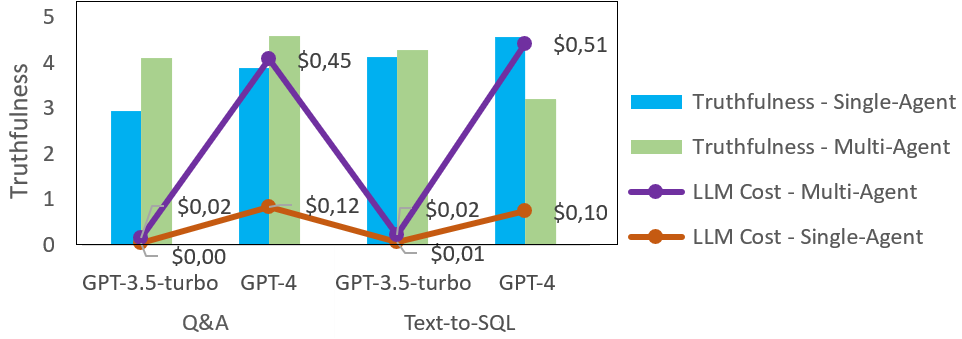
\includegraphics[width=0.75\textwidth]{images/truthfulness_vs_cost_vs_config_model.png}
                    % }
                    \caption{Average LLM costs and Truthfulness per completed task according to setup and model.}
                    \label{fig:truthfulness_vs_cost_vs_config_model}
                \end{figure}
                
                

        \subsection{Discussion} % NEW SUBSECTION for your discussion
            % The original \section{Discussion} and all its content go here.
            % The original \subsections become \subsubsections.

            
            The comparison between single and multi-agent systems revealed significant differences in terms of performance and cost:
            
            \subsubsection{General Performance.}     
                The results indicate that for Q\&A tasks in the context of O\&G, truthfulness measure was 28\% higher with the multi-agent architecture compared to single. 
                However, for Text-to-SQL tasks, this trend was inverted, where the single-agent scored 15\% higher.

                These findings suggest that for Q\&A tasks, the multi-agent setup may be more advantageous in terms of providing truthful information, particularly when utilizing the more advanced GPT-4 model. 
                Conversely, in Text-to-SQL tasks, the GPT-4 model in a single-agent configuration proved more effective. 
                This might imply that the added complexity of managing multiple agents in some tasks does not necessarily lead to improved performance in responses, underscoring the importance of carefully selecting the agent configuration based on the task type and specific features of the language model used.
                    
            \subsubsection{Cost-Performance Analysis.}
                While the multi-agent system shows higher truthfulness in Q\&A tasks, it is crucial to consider the associated costs. 
                To provide a clearer comparison, let us consider the score/cost ratios. For Q\&A tasks using GPT-4, the single-agent configuration yields a ratio of 32.33 truthfulness points per dollar, compared to 10.16 for the multi-agent setup. This indicates that while the multi-agent system shows a 17.8\% improvement in truthfulness, it comes at a 275\% increase in cost.
                
                % Based on our analysis, we recommend using a multi-agent system for Q\&A tasks when the budget allows for it and accuracy is a critical factor. 
                % However, decision-makers should consider setting a cost-performance threshold to guide the choice of system configuration, ensuring that the benefits justify the expenses involved.
                \xexeo{TEm que deduzir a necessidade de fazer um experimento antes levando essas coisas em consideração}
                \vitor{Feito abaixo.}

                This trade-off highlights an important implication for any organization considering the adoption of these technologies. The optimal architecture is not universal; it is highly dependent on specific task requirements and budget constraints. 
                This reality underscores the necessity of conducting a preliminary, cost-performance evaluation. Rather than simply selecting a model, decision-makers must first perform a targeted analysis to establish a cost-benefit threshold. 
                Our work not only provides initial data for the O\&G domain but also demonstrates a foundational methodology for this evaluation process, which ultimately motivated the more rigorous and quantitative approach of our second experimental cycle.


            \subsubsection{Model Performance Variations.}
                Interestingly, our results show that GPT-3.5-turbo outperforms GPT-4 in certain tasks, particularly in the Text-to-SQL multi-agent configuration, despite GPT-4's larger size and more extensive training. 
                This unexpected performance could be attributed to several factors. 
                First, GPT-3.5-turbo may have undergone more specific fine-tuning for structured query tasks, allowing it to excel in Text-to-SQL scenarios. 
                Additionally, GPT-3.5-turbo's training data might be more recent or more relevant to the specific domain of our study. 
                Another possibility is that the smaller model size of GPT-3.5-turbo allows for faster processing and more efficient handling of the multi-agent setup, resulting in better performance in some contexts.

                However, it is important to note that GPT-4, when used in a multi-agent setup, demonstrated more consistent truthfulness and performance, as evidenced by its reduced standard deviation in results. 
                This consistency can be particularly advantageous in applications where reliability and accuracy are critical. 
                Multi-agent systems have the advantage of maintaining separate contexts for different aspects of a task \citep{Langchain2025}. 
                \xexeo{Você pode suportar essa afirmação com uma citação?}
                \vitor{Feito.}
                This compartmentalization can lead to better handling of complex, multi-faceted queries, as each agent can focus on its specific context without being overwhelmed by irrelevant information. However, this advantage may be offset in tasks like Text-to-SQL, where maintaining a unified context of the database schema and query structure is crucial, possibly explaining the better performance of single-agent setups in this task.
                Furthermore, the multi-agent architecture inherently involves multiple stages of information processing, which can serve as natural filtering mechanisms.
                As information passes from one agent to another, irrelevant or low-quality data may be naturally filtered out, leading to more refined and accurate final outputs. 
                This could explain the superior performance in filtering irrelevant information observed in multi-agent setups.
            
            
            \subsubsection{Economic Efficiency.} 
            
                The multi-agent architecture incurs significantly higher costs compared to the single-agent system, primarily due to additional intermediate calls to the language model and multiple iterations between agents for action planning. 
                Also, the cost differences between using GPT-4 and GPT-3.5-turbo are substantial, with GPT-4 being 20 times more expensive (in early 2024).
                \xexeo{Dizer x vezes mais caro em julho de 2025}.
                \vitor{Feito}

                The average cost per query for each configuration is presented in Table \ref{tab:cost_per_query}. These figures highlight the direct cost implications of the chosen architecture and model.
                
                \begin{table}[h!]
                \centering
                \caption{Average LLM Cost Per Query (USD). Values from early 2024.}
                \label{tab:cost_per_query}
                \begin{tabular}{l r}
                \toprule
                \textbf{Configuration} & \textbf{Cost per Query} \\
                \midrule
                Single-Agent (GPT-3.5-Turbo) & \$0.0068 \\
                Single-Agent (GPT-4) & \$0.1095 \\
                Multi-Agent (GPT-3.5-Turbo) & \$0.0197 \\
                Multi-Agent (GPT-4) & \$0.4896 \\
                \bottomrule
                \end{tabular}
                \end{table}

                To illustrate the financial implications of adopting different models and architectures, we estimate the annual costs for a large company with 40,000 knowledge workers. Our calculations are based on an average of 5 queries per worker per day, over 250 working days per year.
                
                Under these assumptions, the total annual query volume is 50 million (40,000 workers $\times$ 5 queries/day $\times$ 250 days). For a single-agent configuration, this results in an annual cost of approximately \$337,843 for GPT-3.5 and \$5.47 million for GPT-4.
                
                In a multi-agent architecture, the costs increase substantially, escalating to approximately \$986,631 for GPT-3.5 and \$24.48 million for GPT-4. These estimates underscore the significant financial trade-offs when adopting a multi-agent system, which, while potentially offering performance benefits, comes with a considerable increase in LLM operational costs.

                While multi-agent systems and more advanced models like GPT-4 offer improvements in performance, the economic efficiency, as measured by truthfulness per dollar, may favor single-agent systems and less costly models like GPT-3.5-turbo, depending on the specific application and budget constraints.

                It is important to note that, as of July 2025, the landscape of LLMs has evolved substantially. The emergence of more efficient models, has led to a significant decrease in API's costs. This suggests that the financial trade-offs discussed previously may no longer be as pronounced, and that high-performance multi-agent systems could become economically viable much sooner than anticipated.

                \xexeo{In summary é o parágrafo típico das LLMs... Mas é isso mesmo. Porém tem que colocar um ponto: o custo dos modelos está caindo barbaramente com o aparecimento de novos modelos no topo de desempenho e novas tecnologias tem permitido alcançar resultados de ótima qualidade com máquinas muito menores, o que também derruba o custo. Pode até citar o exemplo do DeepSeek (buscando na literatura o desempenho x custo dele)}
                \vitor{Feito}
                
            
            \subsubsection{Challenges and Limitations}     
                During the evaluation of the agents, several challenges and limitations were identified.

                \textbf{\textit{Contextualization and Interpretation.}} 
                    In many cases, the single-agent solution had difficulty understanding the context of the question. For example, a question about cementing was interpreted in the context of the construction industry, a theme to which the language models were more exposed during the training phase. 
                    However, the multi-agent structure, with its well-defined roles, better understood the questions and showed superior performance in Q\&A tasks, corroborating the findings of \citep{Li2024}.
                
                \textbf{\textit{Filtering Irrelevant Information.}} 
                    The agent often receives irrelevant documents along with important ones in the prompt context, and it is up to the LLM to ignore these. 
                    For example, when asked about alternatives to accelerate the curing time of cement paste without compromising its integrity at high temperatures, the RAG system retrieved a document that included information about batch cementing to ensure homogeneity during manufacturing and pumping. 
                    While this information is true, it was not relevant to the specific question asked. 
                    In this aspect, the multi-agent solution performed better at discarding such irrelevant information, focusing more accurately on the task at hand. 
                    Other possible solutions include improving the accuracy of semantic search by adjusting a minimum threshold for similarity measures or through re-ranking techniques such as those proposed by \citep{Carraro2024} and \citep{Sun2023}.
                
                \textbf{\textit{Hallucination.}} 
                    During the evaluation of our system, we encountered instances where the agent produced hallucinated information instead of utilizing the appropriate tool to retrieve accurate data, as in \citep{Bilbao2023}. 
                    For example, when asked, "How many anomalies occurred on rig number 05 during August 2023?" the agent was expected to use the Text-to-SQL tool to query the database. 
                    However, it bypassed this tool and generated a fabricated response, stating that 5 anomalies occurred, along with detailed descriptions of fictional events. The correct answer, as retrieved from the database, was that 7 anomalies occurred. This hallucination likely resulted from the agent's reliance on its internal knowledge rather than external data retrieval. 

                    In terms of hallucination statistics, our analysis revealed that for Q\&A tasks, hallucinations occurred in 9.6\% of cases and 3.8\% for partially hallucinated. 
                    In contrast, Text-to-SQL tasks exhibited a lower hallucination rate, with only 3.6\% of responses containing hallucinated information and 96.4\% being accurate. 
                    These findings highlight the variation of susceptibility to hallucination in different types of tasks, highlighting the need for targeted strategies to mitigate this problem.
                
                \textbf{\textit{Industry Jargon:}}
                    Specifically analyzing the activity of drilling and completion of offshore wells, the main challenge is the inherently complex and technical nature of the data involved. 
                    There were instances of incorrect interpretation of information, likely due to the use of terms, expressions, and themes specific to well construction, to which the language model had little or no exposure during training phase. 
                    A possible solution is the implementation of specialized models, which has been pointed out in gray literature as a trend for the coming years \citep{Shah2024, Meena2023, Ghosh2023}.
                
                \textbf{\textit{Tools vs. Performance:}} 
                    It was identified during the experiments that agents with a high amount of tools showed a decline in overall performance. 
                    This can be attributed to the added context to the prompts. 
                    As the context length increases, the model's ability to accurately interpret and respond diminishes.
                    This is a limitation of current language models, where longer contexts can lead to a dilution of relevant information and increased difficulty in maintaining coherence and accuracy. 
                    This conclusion is currently qualitative, as these metrics were not addressed in this experiment.

                
                \textbf{\textit{Queries Involving Proper Names:}}
                    In queries involving people's names, it was not possible to retrieve relevant documents using semantic search. 
                    For example, when asked to identify the employee associated with a specific key and list knowledge items they registered in the system, the LLM incorrectly attributed knowledge items to the wrong author\xexeo{O RAG ou a LLM usando o RAG, não ficou claro}\vitor{OK}. 
                    This highlights the difficulty in accurately retrieving information based on proper names, which can be complicated by variations in accentuation, abbreviation, and formatting.
                    \xexeo{tem evidências disso em outros artigos?}
                    \vitor{não encontrei}
                    A potential solution to be explored is the use of Self-Query Retriever \citep{LangchainSelfQuery2023}, implementing a hybrid search with metadata filters (including proper names) and semantic retrieval of the rest of the query. 
                    It is also suggested, in these cases, to use the \citep{Levenshtein1966} distance to handle possible variations in the spelling of names. 
                    This approach could improve the accuracy of retrieving documents related to specific individuals, ensuring that the correct information is associated with the right person.
                    
            
            % \subsubsection{Practical Implications}
            \subsubsection{Practical Implications.} 

                The findings from our study have significant practical implications for the O\&G sector, and potentially for other industries characterized by complex and technical data environments:
                    
                \begin{itemize}
                
                    \item \textbf{Enhanced Decision-Making Support:}
                        Our results indicate that multi-agent systems provide a 28\% higher truthfulness measure in Q\&A tasks. This can be particularly beneficial for decision-making in well engineering, where accurate and truthful information is critical.
                        Implementing multi-agent systems in decision-making processes can lead to more reliable and informed decisions, thereby reducing the risk of errors and enhancing operational safety and efficiency.
                    
                    \item \textbf{Balancing Performance and Economic Efficiency:}
                        While multi-agent systems offer superior performance in terms of truthfulness, they come with a cost that is 3.7 times higher on average compared to single-agent systems.
                        This highlights the importance of a strategic approach in selecting agent configurations based on specific tasks and budget constraints. 
                        % For instance, single-agent systems might be more cost-effective for Text-to-SQL tasks where they have shown to perform 15\% better. 
                        A detailed cost-benefit analysis reveals that for Q\&A tasks using GPT-4, the single-agent configuration yields a ratio of 32.33 truthfulness points per dollar, compared to 10.16 for the multi-agent setup. While the multi-agent system shows a 17.8\% improvement in truthfulness, this comes at a 275\% increase in cost. The efficiency varies significantly by task type; in Text-to-SQL tasks, the GPT-4 single-agent outperforms the multi-agent by 42.5\% in truthfulness while costing 80.4\% less. 
                        % These quantitative insights emphasize the need for careful consideration of task requirements and budget constraints when choosing between single and multi-agent configurations.
                        
                    \item \textbf{Reflection and Critic Agents:}
                        A promising approach to enhance the performance of these agents is the use of reflection \citep{Shinn2023}, a method where agents verbally reflect on task feedback signals and maintain this reflective text in an episodic memory buffer to improve decision-making in subsequent trials. Critic agents are a way to implement reflection in a multi-agent setup. This type of agent is challenging to apply in Q\&A tasks over private technical data, as commercial LLMs (OpenAI, Google Bard, and others) have not been deeply trained in the domain and struggle to provide relevant and precise critiques, reinforcing the trend toward increased use of domain-specific models \citep{Shah2024, Meena2023, Ghosh2023}.                
                        
                    \item \textbf{Task-Specific Agent Configuration:}
                        The study highlights that the complexity of managing multiple agents does not always lead to better performance. In some cases, a single-agent setup might be more effective.
                        This insight can guide the development and deployment of AI systems, ensuring that the configuration of agents is tailored to the specific requirements of the task, thereby optimizing both performance and cost.           
                        
                    \item \textbf{Potential for Broader Application:}
                        The insights gained from this study are not limited to the O\&G sector but can be applied to other industries with similar technical complexities, such as aerospace, pharmaceuticals, and renewable energy.
                        By adopting multi-agent systems in these industries, organizations can improve decision-making, knowledge management, and operational efficiency, driving innovation and competitiveness.             
                    
                \end{itemize}
                        
                    
            \subsubsection{Future Directions.} 

                This work indicates possible pathways for enhancing RAG architectures in O\&G sector. 
                
                \begin{itemize}
                
                    \item \textbf{Enhancement of IR Semantic Techniques:}
                        There is a critical need to develop more sophisticated semantic search technologies. Future efforts should focus on enhancing the precision of information retrieval by filtering out irrelevant content more effectively. This will ensure that agents can provide more accurate and contextually appropriate responses, crucial for technical domains such as O\&G.
                        
                    \item \textbf{Development of Domain-Specific Models:}
                        Specialized models tailored specifically to the O\&G and other domains, such as biomedical engineering \citep{Pal2024}, could significantly improve the handling of specific jargon and complex technical data, while reducing LLM costs \citep{Arefeen2024}. Future research should aim to develop and train these models to better understand and interpret the unique language and data types found in O\&G, enhancing the overall accuracy of agent responses.
                        
                    \item \textbf{Optimization of Tool Use in Agent Performance:}
                        The relationship between the quantity of tools available to an agent and its performance needs further exploration. Future studies should quantify the impact of tool availability on agent efficacy and efficiency, aiming to optimize tool use without overwhelming the agent or diluting performance quality.
                        
                    \item \textbf{Integration of Advanced Name Recognition Techniques:}
                        Queries involving proper names pose a significant challenge in semantic search. Integrating advanced retrieval techniques, such as Self-Query Retrievers \citep{LangchainSelfQuery2023} and \citep{Levenshtein1966} distance algorithms, could improve the handling of these queries. Future research should focus on enhancing name recognition capabilities to ensure that agents can accurately retrieve and utilize correct information, especially in scenarios where precision is paramount.
                        
                    \item \textbf{Extension to Other Complex Domains:}
                        The potential applications of multi-agent systems are not limited to the O\&G sector. Future research should explore the adaptation and implementation of these systems in other complex and technical domains, such as aerospace, pharmaceuticals, and renewable energy. Investigating how these systems can support decision-making in these areas will provide valuable insights into their versatility and adaptability.
                        
                    \item \textbf{Hybrid Model Experimentation:}
                        Combining the strengths of single and multi-agent systems could yield significant benefits. Future directions should include experimenting with hybrid models that integrate the robustness and depth of multi-agent interactions with the simplicity and efficiency of single-agent systems. This hybrid approach could potentially offer a balanced solution, maximizing performance while managing costs and complexity.
                        

                \end{itemize}
                
                By pursuing these directions, future research can significantly advance the development of multi-agent systems, not only enhancing their application in the O\&G sector but also expanding their utility across various technologically intensive activities.
                    


\chapter{Experimento 2}
    

    \section{Metodologia 2}
        
        ...

        \begin{algorithm}
            \caption{Experiment Execution Loop}
            \begin{algorithmic}[1]
            \Require questions, setups, models
            \Ensure results
            
            \Function{RunExperiment}{}
                \State $results \gets \{\}$
                
                \ForAll{$question \in questions$}
                    \State $ground\_truth \gets question.ground\_truth$
                    
                    \ForAll{$setup \in setups$}
                        \ForAll{$model \in models$}
                            \State $agent \gets \text{InitializeAgent}(setup, model)$
                            \State $response \gets agent.\text{ProcessQuestion}(question)$
                            
                            \State $metrics \gets \text{EvaluateResponse}(response, ground\_truth)$
                            
                            \State $results[question, setup, model] \gets \{$
                            \State \hspace{1cm} $"response": response,$
                            \State \hspace{1cm} $"metrics": metrics,$
                            \State \hspace{1cm} $"execution\_trace": agent.trace$
                            \State $\}$
                        \EndFor
                    \EndFor
                \EndFor
                
                \State \Return $\text{AggregateResults}(results)$
            \EndFunction
            
            \end{algorithmic}
        \end{algorithm}
            
        \subsection{Dataset de Q\&A}

            ...
        
        \subsection{Setups}
        
            \subsubsection{Linear-Flow with Router}        
                ...
            
            \subsubsection{Single-Agent}        
                ...
            
            \subsubsection{Multi-Agent}        
                ...
            
        \subsection{Frameworks utilizados}
        
            ...
            
        \subsection{Avaliação de desempenho}

            [Falar brevemente sobre métricas, prompts, citar ragas, etc]
            



    \section{Methodology (generated)}

        \subsection{1. Overview}

            This chapter describes the experimental methodology used to evaluate large language model (LLM) agents and workflows for answering questions in the oil well operations domain. The experiment integrates multiple LLM configurations, agent architectures, and retrieval-augmented generation (RAG) tools, leveraging Petrobras datasets.

            \textit{<insert brief summary of research objectives and hypotheses here>}

        \subsection{2. Experimental Workflow (Expanded)}

            \subsubsection{2.1 Dataset Preparation}

            The experimental workflow was designed to provide a thorough and reproducible evaluation of language model agents within oil well operations. The process begins with the careful preparation of the dataset, which is composed of questions and corresponding ground truth answers derived from a diverse range of operational records, incident reports, and lessons learned. To ensure the quality and relevance of the data, questions undergo a filtering and preprocessing phase where clarity, diversity, and alignment with real-world scenarios are prioritized. This includes removing duplicates, standardizing terminology, and confirming that each question is properly paired with an accurate answer. The dataset is further validated for completeness and consistency, ensuring it represents the full spectrum of operational challenges, such as safety, cementing, and intervention scenarios.

            \subsubsection{2.2 Model and Setup Selection}

            Following dataset preparation, the experimental design incorporates a variety of agent architectures. These include approaches where questions are routed to specialized agents, single-agent systems that centralize all reasoning and retrieval, and multi-agent frameworks that leverage collaboration among specialized agents under a supervisory structure. Each of these configurations is evaluated using different language models, allowing for a comprehensive assessment of how model choice and agent setup influence performance. The agents are also provided with access to advanced retrieval tools and domain-specific knowledge bases, enabling them to draw on a broad foundation of operational expertise.

            \subsubsection{2.3 Execution Loop}

            The core of the experimental workflow is an automated execution loop. For each combination of question, agent setup, and language model, the system systematically loads the relevant data, configures the agent, and executes the workflow. Throughout this process, all responses and intermediate reasoning steps are meticulously logged. This approach not only ensures systematic coverage of all experimental conditions but also provides full traceability for subsequent analysis. The automation of these procedures guarantees consistency and reproducibility, while the comprehensive logging facilitates in-depth evaluation and comparison of agent performance across a range of operational scenarios.

            \subsubsection{2.4 Evaluation and Metrics}

            Following the execution of all experimental combinations, a comprehensive evaluation framework is applied to assess agent performance. The system calculates a suite of quantitative metrics for each question, setup, and model combination by comparing the generated answers against the established ground truth. These metrics include standard performance indicators such as accuracy, precision, recall, and F1 score, which provide a multifaceted view of response quality. For open-ended questions where binary correctness measures are insufficient, a confusion matrix approach is implemented to capture nuances in answer quality and content coverage. Additionally, the system measures answer size ratio relative to ground truth, offering insights into model verbosity and conciseness. These metrics are then aggregated across different dimensions to enable meaningful comparisons between agent architectures and language models, revealing patterns in performance across various operational scenarios and question types.

            \subsubsection{2.5 Reproducibility and Quality Control}

            To ensure scientific rigor and reproducibility, the experimental methodology incorporates robust tracking of all environmental variables and configuration parameters. The system maintains detailed logs of the computational environment, including software versions, dependency specifications, and hardware characteristics that might influence results. All experimental parameters, from model identifiers to dataset specifications, are systematically recorded alongside the results they generate. Throughout the experimental process, periodic validation checks are performed to maintain data integrity and result consistency, with anomalies flagged for investigation. This comprehensive approach to reproducibility not only facilitates verification of findings but also enables future extensions of the research with comparable baselines. The quality control measures embedded in the workflow ensure that conclusions drawn from the experiments rest on a foundation of methodological soundness and data reliability.

            \textit{<insert workflow diagram or pseudocode here to illustrate the above stages>}

        \subsection{3. Data Sources}

            The experimental evaluation relies on a carefully curated collection of data sources that represent the diverse knowledge domains relevant to oil well operations. At the core of the experiment is a comprehensive questions dataset containing structured entries that simulate real-world queries an operator might encounter. This dataset was developed through extensive collaboration with domain experts and analysis of historical operational records. Each entry in the dataset contains a question formulated in natural language, a unique identifier, categorical metadata to facilitate analysis, and a corresponding ground truth answer validated by subject matter experts. The questions span various complexity levels, from factual inquiries to complex reasoning scenarios that require integration of multiple knowledge sources.

            To provide the language models with the necessary domain knowledge, the experiment incorporates several specialized knowledge bases that reflect different aspects of oil well operations:

            \begin{itemize}
                \item \textbf{Knowledge Bases and Tools}:
                \begin{itemize}
                    \item \textbf{Lessons}: A repository of knowledge items capturing insights, best practices, and technical know-how from past oil well operations. These lessons represent institutional memory and expertise accumulated over years of operational experience.
                    \item \textbf{Alertas SMS}: A collection of safety alerts and incident reports documenting past events, near-misses, and accidents, providing critical safety information and preventative measures.
                    \item \textbf{Cronoweb}: A comprehensive database of scheduling information and intervention records, detailing maintenance activities, equipment deployments, and operational timelines.
                    \item \textbf{SITOP}: Detailed daily operational logs from drilling rigs, containing technical parameters, operational decisions, and situational reports from active drilling operations.
                \end{itemize}
            \end{itemize}

            These knowledge sources were preprocessed to ensure consistency, remove sensitive information, and optimize retrieval performance. The integration of these diverse data sources enables a holistic evaluation of how language model agents navigate the complex informational landscape of oil well operations, from technical specifications to safety protocols and historical precedents.

            \textit{<insert table or image summarizing datasets and tools here>}

        \subsection{4. System Architecture}

            The experimental system was implemented using modern Python frameworks specialized for language model orchestration and agent workflows. The architecture leverages the LangChain and LangGraph ecosystems, which provide robust foundations for building complex language model applications with multiple components and state management. This subsection details the modular design of the system, highlighting how different components interact to enable systematic evaluation of language model agents in oil well operations.

            \subsubsection{4.1 Experiment Orchestration}

            At the core of the system architecture is an experiment orchestration layer responsible for coordinating the entire evaluation process. This component manages the loading of questions from the dataset, systematically iterates through different model and setup combinations, and ensures proper logging of results. The orchestrator maintains experiment state across multiple runs, handles error recovery, and implements checkpointing to allow for resumption of long-running experiments. By centralizing control flow, this component ensures that all experimental conditions are tested consistently and that results are captured in a standardized format for subsequent analysis.

            \subsubsection{4.2 Agent Workflow Frameworks}

            The system implements multiple agent workflow frameworks to evaluate different approaches to question answering in the oil well domain. These frameworks define the flow of information and decision-making processes within and between language model agents. The implemented workflows include a Linear-Flow with Router (CORTEX) that directs questions to specialized processing paths, a Single-Agent approach that centralizes all reasoning and tool use, and a Multi-Agent Supervisor framework that coordinates multiple specialized agents. Each workflow is defined declaratively, specifying the sequence of operations, decision points, and information exchange patterns that govern agent behavior during question processing.

            \subsubsection{4.3 Nodes and Tool Integration}

            The system architecture includes specialized nodes that implement specific reasoning steps and tool-calling logic. These nodes serve as the building blocks of agent workflows, encapsulating discrete functionality such as question analysis, knowledge retrieval, and answer synthesis. The tool integration layer provides agents with access to external knowledge sources through a standardized interface, enabling semantic search over domain-specific corpora, structured data queries, and other specialized operations. This modular approach to tool integration allows for consistent evaluation of how different agent architectures leverage available tools and knowledge sources.

            \subsubsection{4.4 Prompt Engineering and System Messages}

            A critical component of the architecture is the prompt engineering layer, which defines the instructions and context provided to language models. This includes carefully crafted system messages that establish the role and capabilities of each agent, prompt templates that structure inputs consistently across experimental conditions, and few-shot examples that guide model behavior. The system maintains a library of prompt variants optimized for different tasks within the question-answering workflow, ensuring that each agent receives appropriate guidance while maintaining experimental control.

            \subsubsection{4.5 State Management and Metrics}

            The architecture incorporates a comprehensive state management system that tracks the progress of experiments, maintains contextual information across agent interactions, and captures intermediate reasoning steps. This component is tightly integrated with the metrics calculation subsystem, which computes performance indicators in real-time as experiments progress. The metrics framework implements various evaluation approaches, from simple accuracy measures to sophisticated semantic similarity calculations, providing multi-dimensional assessment of agent performance. All experimental data, including intermediate states and final results, is persisted in structured formats to enable both immediate feedback and in-depth post-experiment analysis.

            \textit{<insert system architecture diagram here>}

        \subsection{Experimental Setups}

            To comprehensively evaluate language model performance in well construction operations, the experiment employed multiple agent architectures and model configurations. This subsection details the different experimental setups, highlighting their design principles, operational characteristics, and the rationale behind their selection. The experimental design deliberately incorporates contrasting approaches to agent architecture, enabling comparative analysis of different strategies for complex question answering in specialized domains.
            

            \subsubsection{Linear-Flow}

                The Linear-Flow architecture represents the simplest RAG design, where user input is processed in a strictly sequential manner. 

                \begin{figure}[h]
                    \centering
                    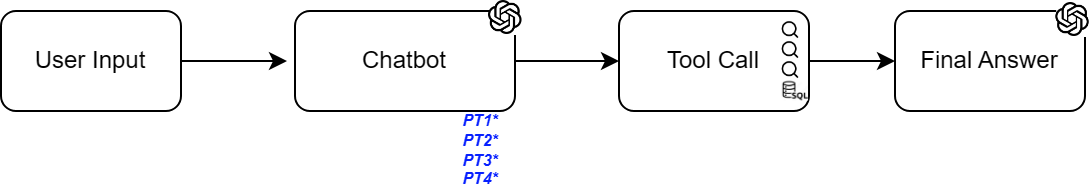
\includegraphics[width=0.8\textwidth]{images_exp2/diagrama_linear_flow.png}
                    \caption{Linear-Flow architecture. PT1 indicates Prompt for Tool 1 and so on.}
                    \label{fig:diagrama_linear_flow}
                \end{figure}
           

            \subsubsection{Linear-Flow with Router}

                The Linear-Flow with Router paradigm extends the basic linear flow by introducing a routing mechanism that enables the distribution of tool instruction prompts. As illustrated in Figure~\ref{fig:diagrama_linear_w_router}, instead of a single chatbot generating one query and invoking a single tool, the router decomposes the user input into multiple sub-queries. Each sub-query is then processed independently, often in parallel, by separate tool invocations.
                    
                This approach offers several advantages:
                \begin{itemize}
                    \item \textbf{Increased Throughput:} By distributing sub-tasks across multiple tools, the system can handle more complex or multi-faceted user requests efficiently.
                    \item \textbf{Specialization:} Each tool can be tailored to address a specific aspect of the user's query, allowing for more accurate and relevant results.
                    \item \textbf{Scalability:} The architecture naturally supports scaling, as additional tools can be added to handle more sub-queries or specialized tasks.
                \end{itemize}
                
                In practice, the router acts as an orchestrator, analyzing the user input and generating multiple targeted queries (PT1*, PT2*, PT3*, PT4* in the figure). These queries are dispatched to their respective tools, and the results are aggregated to form the final answer. This method is particularly effective for tasks that can be decomposed into independent components, such as multi-part questions or workflows requiring different types of expertise.
                
                Compared to the standard linear flow, the use of a router introduces additional complexity in query generation and result aggregation but enables a significant boost in system flexibility and performance.

                \begin{figure}[h]
                    \centering
                    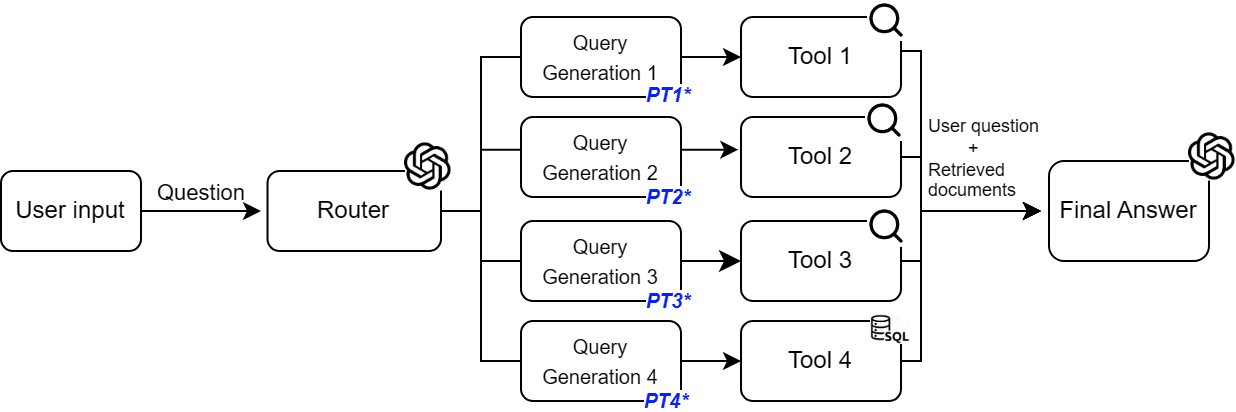
\includegraphics[width=0.8\textwidth]{images_exp2/diagrama_linear_w_router.png}
                    \caption{Linear-Flow with Router architecture.}
                    \label{fig:diagrama_linear_w_router}
                \end{figure}
                
                

                
            \subsubsection{Single-Agent}

                The Single-Agent approach represents a centralized architecture where a single language model agent handles the entire question-answering process. This agent has access to the full suite of retrieval tools and knowledge sources, making independent decisions about which tools to invoke and how to synthesize information into coherent answers. The design emphasizes end-to-end reasoning within a unified context, allowing the model to maintain a consistent understanding throughout the process. This approach tests the capability of language models to manage complex workflows autonomously, balancing between exploration of different knowledge sources and focused answer generation without the overhead of inter-agent communication.
                
                \begin{figure}[h]
                    \centering
                    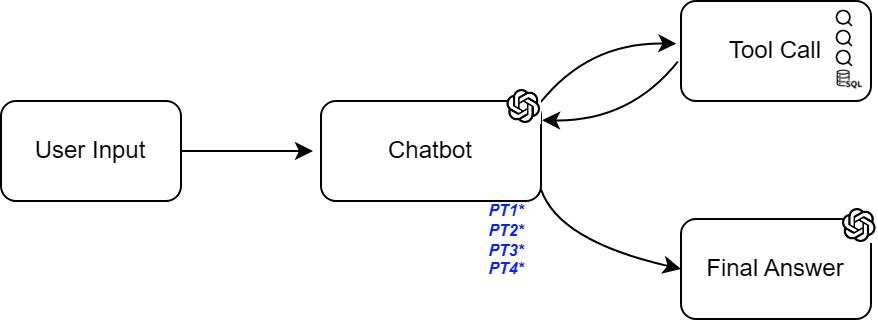
\includegraphics[width=0.8\textwidth]{images_exp2/diagrama_single_agent.png}
                    \caption{Single-Agent architecture}
                    \label{fig:diagrama_single_agent}
                \end{figure}


            \subsubsection{Multi-Agent Supervisor}

                The Multi-Agent Supervisor setup implements a collaborative approach where multiple specialized agents work together under the coordination of a supervisor agent. Each specialized agent focuses on a specific domain of knowledge or reasoning skill, such as retrieval, analysis, or explanation generation. The supervisor agent orchestrates the collaboration, delegating subtasks to appropriate specialized agents, integrating their contributions, and ensuring coherence in the final answer. This architecture explores the potential benefits of distributed cognition, where complex reasoning is decomposed into manageable components handled by purpose-built agents. The framework includes mechanisms for resolving conflicts between agents and synthesizing potentially divergent perspectives into unified responses.

                \begin{figure}[h]
                    \centering
                    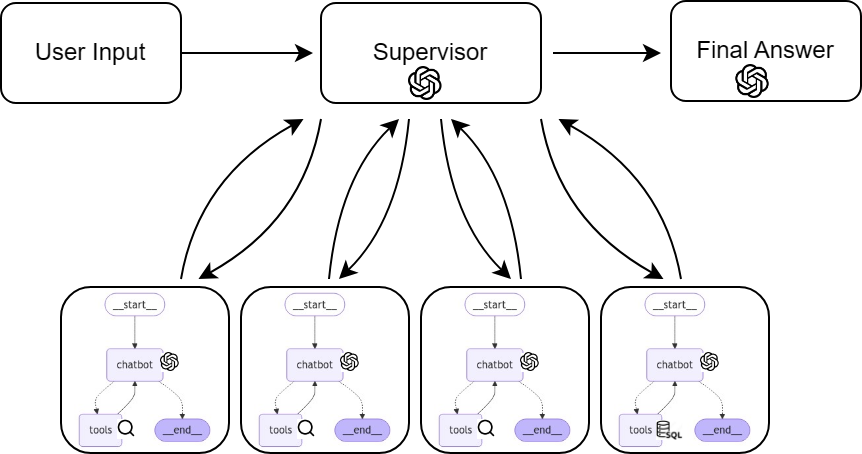
\includegraphics[width=0.8\textwidth]{images_exp2/diagrama_multiagente_supervisor.png}
                    \caption{Multi-Agent setup with one supervisor and 4 specialist agents.}
                    \label{fig:diagrama_multiagente_supervisor}
                \end{figure}


                \textit{<insert table summarizing experimental setups and models here>}

        \subsection{6. Execution Details}

            The experiment was driven by a script without manual intervention during the evaluation process. A main execution loop systematically iterated through all combinations of questions, agent setups, and language models defined in the experimental design. 

            \subsubsection{6.1 Tool Integration and Knowledge Access}

            During execution, the agent systems accessed domain-specific knowledge through a standardized tool interface layer. This layer provided consistent access patterns across all experimental configurations, ensuring that differences in performance could be attributed to agent architecture rather than variations in knowledge availability. The tool integration framework supported a diverse range of knowledge access methods, including semantic search over unstructured text corpora, structured queries against relational databases, and specialized information extraction routines tailored to the oil well operations domain. Each tool invocation was executed within a controlled environment that captured performance metrics such as latency and resource utilization, providing additional dimensions for analysis beyond answer correctness. The standardization of tool interfaces across agent architectures was a critical design decision that enabled fair comparison while still allowing each architecture to implement its own strategy for tool selection and result interpretation.

            \subsubsection{6.2 Comprehensive Logging and Observability}

            A cornerstone of the experimental methodology was the implementation of comprehensive logging throughout the execution process. The system captured detailed records of each step in the question-answering workflow, from initial question parsing to final answer generation. These logs included intermediate reasoning steps, tool invocations with their inputs and outputs, and internal state transitions within the agent systems. All experimental artifacts were persisted in structured formats that facilitated both automated analysis and manual inspection. The logging system implemented a hierarchical organization that linked high-level metrics to the detailed execution traces that produced them, enabling root cause analysis of performance patterns. This observability infrastructure was essential for understanding not just what results were produced, but how and why different agent architectures arrived at their answers, providing insights into their reasoning processes and failure modes.

            \textit{<insert code snippet or pseudocode of main execution loop here>}

        \subsection{7. Evaluation Metrics}

            The evaluation of each experimental run is grounded in a comprehensive set of metrics designed to capture both the correctness and the quality of the system’s responses. Standard quantitative measures such as accuracy, precision, recall, and F1 score are calculated by comparing the answers generated by the agent systems to the established ground truth for each question. These metrics provide a multifaceted view of performance, indicating not only how often the system produces correct answers but also how well it balances false positives and false negatives.

            For questions that are open-ended or less amenable to binary correctness, the evaluation framework employs a confusion matrix approach. This allows for a more nuanced assessment, capturing partial correctness and the degree to which the system’s response overlaps with the expected content. Additionally, the methodology includes the calculation of the answer size ratio, which measures the verbosity of the generated answer relative to the ground truth. This metric helps to identify tendencies toward overly concise or excessively verbose responses, offering further insight into the models’ behavior and suitability for practical deployment.

        \subsection{8. Reproducibility}

            Ensuring reproducibility is a cornerstone of the experimental methodology. To this end, every aspect of the computational environment is meticulously documented. This includes recording the exact Python version used, as well as all package dependencies and their respective versions. Hardware specifications, such as processor type and available memory, are also logged to account for any potential influence on experimental outcomes.

            Beyond the environment, the system systematically records all configuration parameters relevant to each experimental run. This encompasses model names, hyperparameters, and dataset paths, as well as any other settings that might affect the results. By maintaining this comprehensive record, the methodology enables other researchers to replicate the experiments precisely or to build upon them with confidence that baseline conditions are well understood and controlled.

        \subsection{9. Limitations}

            While the experimental methodology strives for rigor and comprehensiveness, several limitations must be acknowledged. One key limitation concerns the coverage of the dataset: although the question set is carefully curated to represent a broad range of operational scenarios, it may not capture the full diversity of real-world challenges encountered in oil well operations. Similarly, the models and agent architectures evaluated are constrained by the available computational resources and the current state of language modeling technology, which may limit their ability to generalize beyond the scenarios tested.

            Another limitation arises from the reliance on ground truth answers, which, despite expert validation, may still reflect subjective judgments or incomplete information in certain cases. Furthermore, the evaluation metrics, while robust, may not fully capture qualitative aspects of answer usefulness or clarity, especially in highly technical or ambiguous situations. Recognizing these limitations is essential for interpreting the results and for guiding future research aimed at addressing these gaps.

        \subsection{10. Summary}

            This methodology provides a systematic framework for comparing different agent architectures and large language models in the context of complex question answering for oil well operations. By integrating rigorous evaluation metrics, robust reproducibility practices, and a clear acknowledgment of limitations, the approach enables meaningful insights into the strengths and weaknesses of various system designs. The findings derived from this methodology can inform both the deployment of language model agents in operational settings and the ongoing development of more capable and reliable AI systems for specialized industrial domains.


    \section{Resultados e Discussão}

        
        \subsection{Performance}

        
            [GERAR TEXTO AQUI]

            ...

            ...
            
            ...

            [GERAR GRÁFICO NOVO AQUI onde config são as cores e X os modelos]
            
            \begin{figure}[h!]
                \centering              
                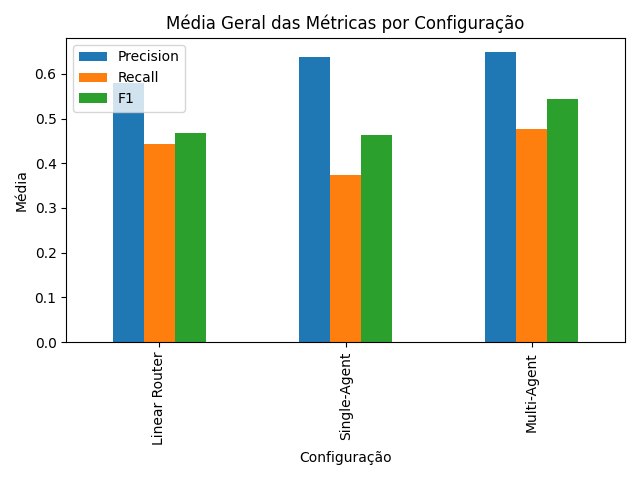
\includegraphics[width=0.75\textwidth]{images_part_2/media_geral_por_configuracao.png}
                \caption{Precisão, recall e f1 por configuração.             [GERAR GRÁFICO NOVO AQUI]}
                \label{fig:aaaa}
            \end{figure}


            ...
            
            ...

            ...
        
            \subsubsection{F1 Score}
            
                
                [GERAR TEXTO AQUI]

                ...

                ...

                ...
                
                % \begin{figure}
                %     \centering
                %     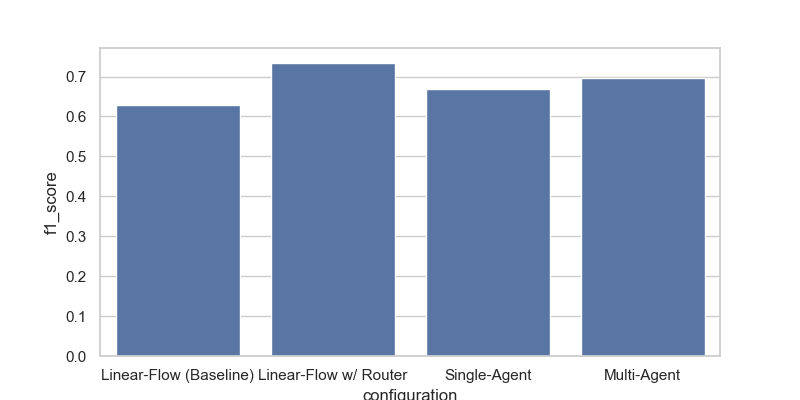
\includegraphics[width=0.5\linewidth]{images_exp2/bar_avg_f1_by_configuration.png}
                %     \caption{Average F1 by RAG architecture.}
                %     \label{fig:enter-label}
                % \end{figure}

                % \begin{figure}
                %     \centering
                %     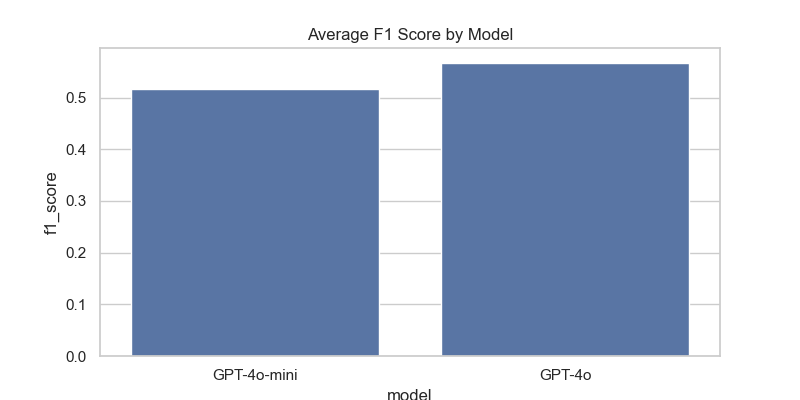
\includegraphics[width=0.5\linewidth]{images_exp2/bar_avg_f1_by_model.png}
                %     \caption{Average F1 Score by language model.}
                %     \label{fig:enter-label}
                % \end{figure}            
                \begin{figure}[h]
                \centering
                \begin{minipage}{0.45\textwidth}
                    \centering
                    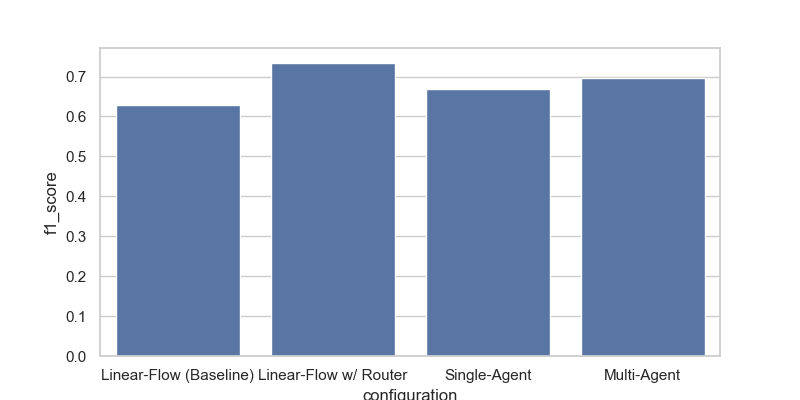
\includegraphics[width=\textwidth]{images_exp2/bar_avg_f1_by_configuration.png}
                    \caption{Image 1 caption}
                    \label{fig:image1}
                \end{minipage}
                \hfill
                \begin{minipage}{0.45\textwidth}
                    \centering
                    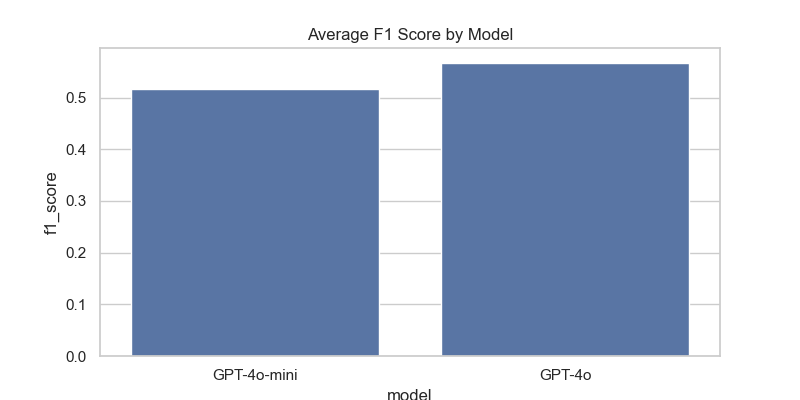
\includegraphics[width=\textwidth]{images_exp2/bar_avg_f1_by_model.png}
                    \caption{Image 2 caption}
                    \label{fig:image2}
                \end{minipage}
                \end{figure}
                
                
                [GERAR TEXTO AQUI]

                ...

                ...

                ...
                % \begin{figure}[h!]
                %     \centering              
                %     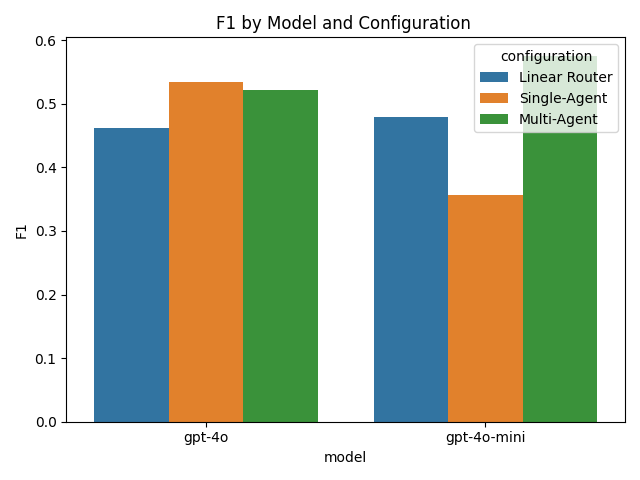
\includegraphics[width=0.75\textwidth]{images_part_2/model_f1_model_configuration.png}
                %     \caption{F1 Score por modelo e configuração.}
                %     \label{fig:aaaa}
                % \end{figure}
                \begin{figure}
                    % \centering
                    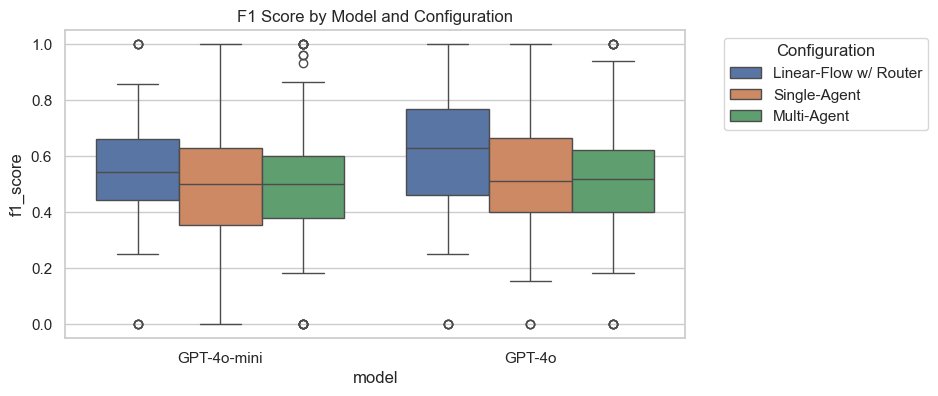
\includegraphics[width=1.1\linewidth]{images_exp2/f1_score_by_model_and_configuration.png}
                    \caption{F1 Score distribution by model and configuration of agents}
                    \label{fig:f1_score_by_model_and_configuration}
                \end{figure}
                    
                [GERAR TEXTO AQUI]

                ...

                ...

                ...
                
                
                \begin{figure}
                    \centering
                    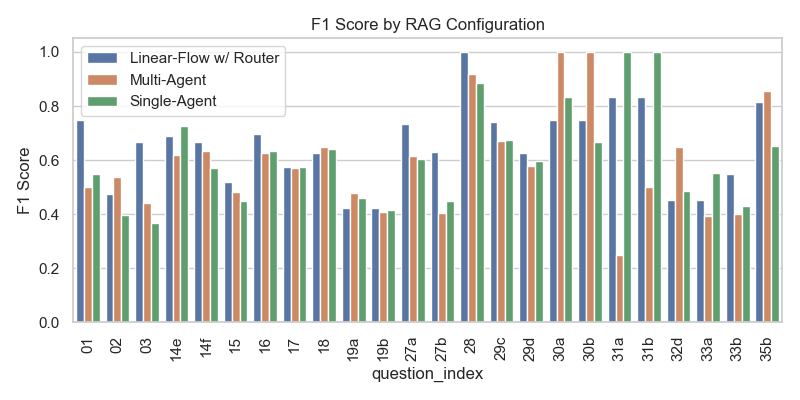
\includegraphics[width=1\linewidth]{images_exp2/best_f1_by_question_index_and_configuration.png}
                    \caption{Enter Caption}
                    \label{fig:enter-label}
                \end{figure}
                
                [GERAR TEXTO AQUI]

                ...

                ...

                ...
                
                % \begin{figure}[h!]
                %     \centering              
                %     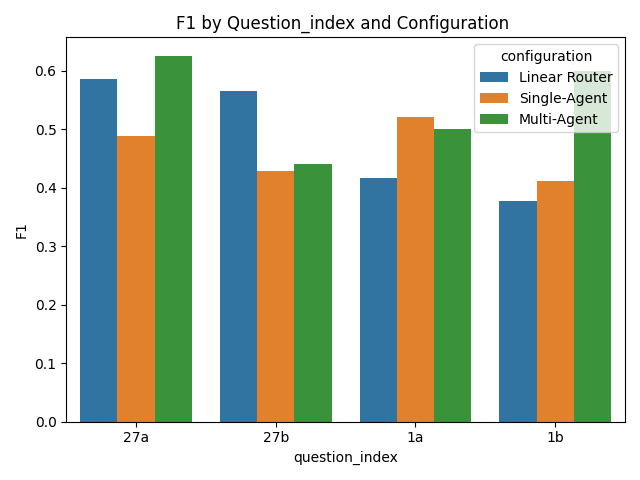
\includegraphics[width=0.75\textwidth]{images_part_2/question_f1_question_index_configuration.png}
                %     \caption{F1 Score por pergunta e configuração.}
                %     \label{fig:aaaa}
                % \end{figure}


                [GERAR TEXTO AQUI]

                ...

                ...
                
                ...

                
                \begin{figure}
                    \centering
                    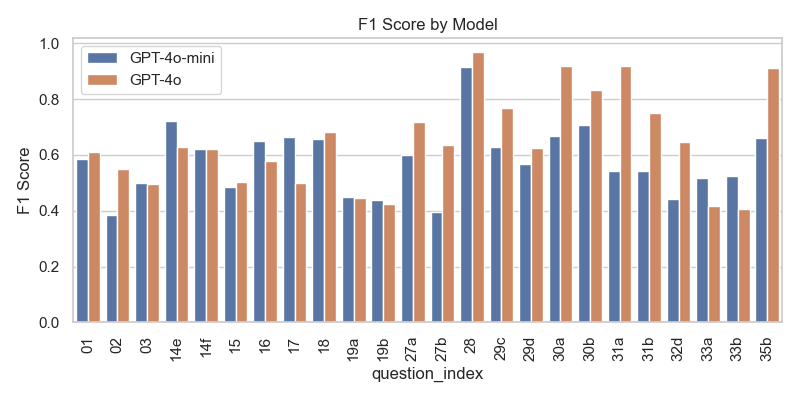
\includegraphics[width=1\linewidth]{images_exp2/best_f1_by_question_index_and_model.png}
                    \caption{Enter Caption}
                    \label{fig:enter-label}
                \end{figure}


            \subsubsection{Precisão}

                [GERAR TEXTO AQUI]

                ...

                ...

                ...

                \begin{figure}[h!]
                    \centering              
                    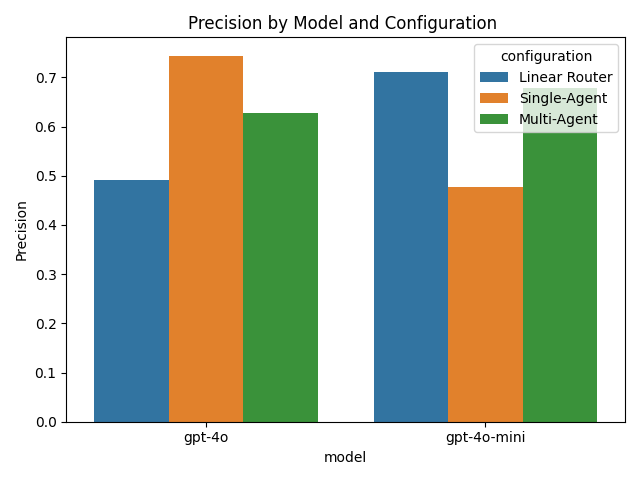
\includegraphics[width=0.75\textwidth]{images_part_2/model_precision_model_configuration.png}
                    \caption{Precisão por modelo e configuração.}
                    \label{fig:aaaa}
                \end{figure}
                
                [GERAR TEXTO AQUI]

                ...

                ...

                ...

                \begin{figure}[h!]
                    \centering              
                    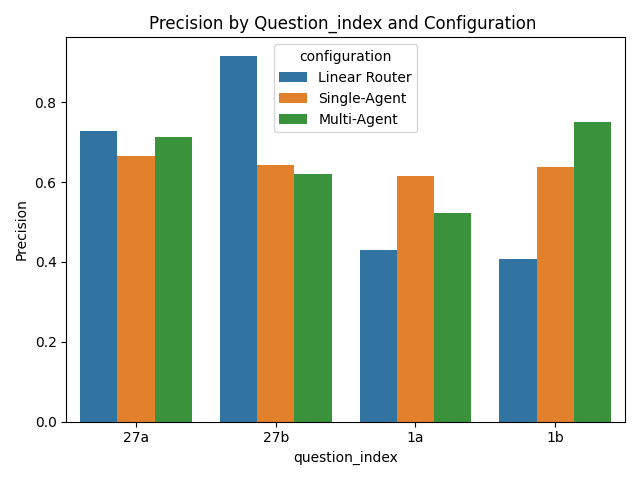
\includegraphics[width=0.75\textwidth]{images_part_2/question_precision_question_index_configuration.png}
                    \caption{Precisão por pergunta e configuração.}
                    \label{fig:aaaa}
                \end{figure}    

                [GERAR TEXTO AQUI]

                ...

                ...

            
            \subsubsection{Recall}
            
                [GERAR TEXTO AQUI]

                ...

                ...
                
                \begin{figure}[h!]
                    \centering              
                    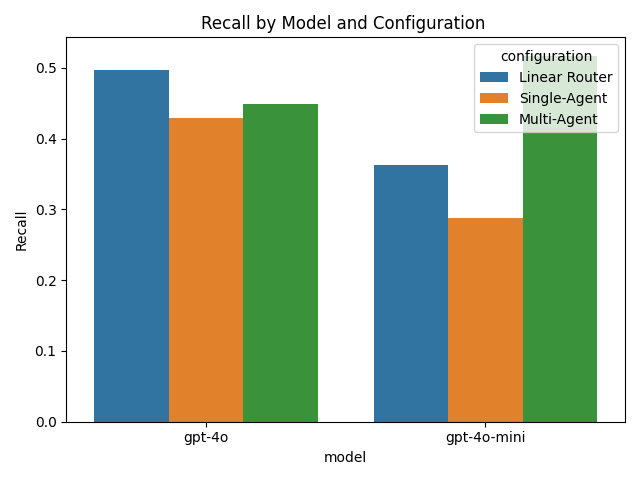
\includegraphics[width=0.75\textwidth]{images_part_2/model_recall_model_configuration.png}
                    \caption{Recall por modelo e configuração.}
                    \label{fig:aaaa}
                \end{figure}

                [GERAR TEXTO AQUI]

                ...

                ...

                ...
                
                \begin{figure}[h!]
                    \centering              
                    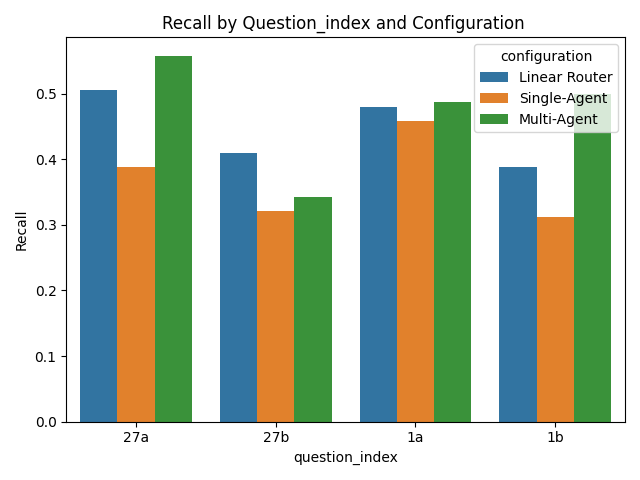
\includegraphics[width=0.75\textwidth]{images_part_2/question_recall_question_index_configuration.png}
                    \caption{Recall por pergunta e configuração.}
                    \label{fig:aaaa}
                \end{figure}

                [GERAR TEXTO AQUI]

                ...

                ...
            

        \subsection{Linear-Flow}


            In this setup, the user’s query is handled by a single LLM step, which carries all the instructions (PT1, PT2, PT3 and PT4, as depicted in \ref{fig:diagrama_linear_flow}) required for the generation of various types of search queries. These instruction prompts are often quite long, as they are carefully crafted to produce high-quality queries for the vector store. Due to the aggregation of all instruction prompts within a single LLM invocation, the resulting context becomes notably extensive. This can lead to performance degradation as the context length increases [O QUE PODE SER VISTO NO GRAFICO TAL EM CONTRASTE COM O SETUP TAL QUE DIVIDE OS PROMPTS EM PARTES]. 
            
            ...

            ...
            
            ...

        \subsection{Linear-Flow with Router}

            [GERAR TEXTO AQUI]

            ...

            ...
            
            ...

        \subsection{Single-Agent}

            [GERAR TEXTO AQUI]

            ...

            ...
            
            ...
        
        \subsection{Multi-Agent}

            [GERAR TEXTO AQUI]

            ...
            
            ...
            
            ...




\chapter{Conclusões 1}

    Os resultados deste estudo destacam o potencial das arquiteturas multiagente baseadas em LLMs no setor de O\&G, especialmente no domínio da engenharia de poços. A capacidade de processar e responder a consultas complexas abre caminho para uma transformação digital significativa na área.
    
    Nossa análise comparativa de arquiteturas de agente único e multiagente, utilizando GPT-3.5-turbo e GPT-4, revela um panorama detalhado de trade-offs entre desempenho e eficiência econômica. Os sistemas multiagente demonstram uma veracidade 28\% maior em tarefas de perguntas e respostas (Q\&A), especialmente com GPT-4, em comparação com sistemas de agente único. No entanto, eles incorrem em custos de LLM que são, em média, 3,7 vezes maiores devido às complexidades da comunicação entre agentes. Em contraste, os sistemas de agente único se destacam em tarefas de Text-to-SQL, apresentando um desempenho 15\% melhor do que as configurações multiagente. Essa dinâmica de custo-benefício exige uma consideração cuidadosa ao implementar RAG em cenários do mundo real, onde precisão e restrições financeiras devem ser equilibradas.
    
    Destacamos vários desafios encontrados durante nossos experimentos, incluindo questões de contextualização, necessidade de filtragem de informações mais refinada e a persistência de alucinações. Esses desafios sublinham a necessidade de pesquisas contínuas em áreas como modelos especializados em domínios específicos, técnicas avançadas de busca semântica e arquiteturas híbridas que combinem as forças dos sistemas de agente único e multiagente.
    
    As implicações práticas deste estudo vão além do setor de O\&G. Os insights alcançados aqui são aplicáveis a qualquer domínio intensivo em conhecimento que lide com grandes volumes de dados técnicos. Ao focar em aprimorar os mecanismos de recuperação, desenvolver LLMs específicos de domínio e otimizar as interações entre agentes e ferramentas, pavimentamos o caminho para soluções RAG mais eficazes, confiáveis e econômicas em diversos setores.
    
    Os principais pontos do estudo são os seguintes: sistemas multiagente oferecem superior veracidade em tarefas de Q\&A, embora a um custo significativamente maior. Arquiteturas de agente único, por outro lado, se destacam em tarefas de Text-to-SQL. Apesar das vantagens, persistem vários desafios, incluindo questões de contextualização, filtragem, alucinação e vocabulário específico de domínio.
    
    Pesquisas futuras devem focar no desenvolvimento de modelos especializados, no avanço das técnicas de recuperação e na exploração de arquiteturas híbridas. As lições aprendidas deste estudo têm implicações mais amplas e podem se estender a outros domínios técnicos complexos. Ao abordar as limitações identificadas neste estudo e abraçar as tendências emergentes em sistemas multiagente e tecnologia RAG, podemos desbloquear seu potencial total, revolucionando a tomada de decisões, a gestão do conhecimento e a eficiência operacional em indústrias complexas em todo o mundo.
    
    


\chapter{Conclusões 2 AAA}

    ...




    

\backmatter
\bibliographystyle{coppe-unsrt}
\bibliography{bib}

\appendix


\chapter{Um apêndice}

    Segundo a norma da ABNT (Associação Brasileira de Normas Técnicas), a definição e utilização de apêndices e anexos seguem critérios específicos para a organização de documentos acadêmicos e técnicos.
    
    Apêndice: O apêndice é um texto ou documento elaborado pelo autor do trabalho com o objetivo de complementar sua argumentação, sem que seja essencial para a compreensão do conteúdo principal do documento. O uso de apêndices é indicado para incluir dados detalhados como questionários, modelos de formulários utilizados na pesquisa, descrições extensas de métodos ou técnicas, entre outros. Os apêndices são identificados por letras maiúsculas consecutivas, travessão e pelos respectivos títulos. A inclusão de apêndices visa a fornecer informações adicionais que possam ajudar na compreensão do estudo, mas cuja presença no texto principal poderia distrair ou desviar a atenção do leitor dos argumentos principais.


\renewcommand{\appendixname}{Anexo}
\appendix


\chapter{Um Anexo}
    Segundo a norma da ABNT (Associação Brasileira de Normas Técnicas), a definição e utilização de apêndices e anexos seguem critérios específicos para a organização de documentos acadêmicos e técnicos.
    
    Anexo: O anexo, por sua vez, consiste em um texto ou documento não elaborado pelo autor, que serve de fundamentação, comprovação e ilustração. O uso de anexos é apropriado para materiais como cópias de artigos, legislação, documentos históricos, fotografias, mapas, entre outros, que tenham relevância para o entendimento do trabalho do autor. Assim como os apêndices, os anexos são identificados por letras maiúsculas consecutivas, travessão e pelos respectivos títulos. Eles são utilizados para enriquecer o trabalho com informações de suporte, garantindo que o leitor tenha acesso a documentos complementares importantes para a validação dos argumentos apresentados no texto principal.

\end{document}

%% 
%%
%% End of file `example.tex'.
